\documentclass[specialist, substylefile = spbu.rtx,
			   subf, href, 12pt]{disser}
			   
\usepackage[a4paper, includefoot,
			left=3cm, right=1.5cm,
			top=2cm, bottom=2cm,
			headsep=1cm, footskip=1cm]{geometry}

\usepackage{cmap}
\usepackage[T2A]{fontenc}
\usepackage[utf8]{inputenc}
\usepackage[english,russian]{babel}
\usepackage{amssymb, amsfonts, amsmath, amsthm} % математические дополнения от АМС
\usepackage{graphicx}
% Включать подсекции в оглавление
\setcounter{tocdepth}{2}

\graphicspath{{images/}{code_snippets/}}
\DeclareGraphicsExtensions{.png,.jpg}

\newcommand\eqdef{\mathrel{\stackrel{\makebox[0pt]{\mbox{\normalfont\tiny def}}}{=}}}
\newtheorem{algorithm}{Алгоритм}



\begin{document}

\institution{%
	Санкт-Петербургский государственный университет\\
	Прикладная математика и информатика
}

\title{Выпускная квалификационная работа}

% Тема
\topic{Обнаружение разладки с помощью метода SSA}

% Автор
\author{Кононыхин Иван Александрович}
\group{%
	Уровень образования: магистратура\\
	Направление 01.04.02 <<Прикладная математика и информатика>>\\
	Основная образовательная программа ВМ.5751.2020 <<Математическое моделирование, программирование и искусственный интеллект>>
}

% Научный руководитель
\sa       {Голяндина Нина Эдуардовна\\%
	Кафедра статистического моделирования}
\sastatus {к.\,ф.-м.\,н., доцент}

% Рецензент
\rev      {А.\,Н.~Пепелышев}
\revstatus{Лектор\\
	к.\,ф.-м.\,н.}

% Город и год
\city{Санкт-Петербург}
\date{2022}

\maketitle

\institution{%
	Saint Petersburg State University \\
	Applied Mathematics and Computer Science \\
	Statistical Modelling
}

\title{Graduation Project}

% Тема
\topic{Heterogeneity detection using SSA method}

% Автор
\author{Kononykhin Ivan Aleksandrovich}
\group{группа 20.М03-мм}

% Научный руководитель
\sa       {N.\,E.~Golyandina}
\sastatus {PhD, Assistant Professor, Department of Statistical Modelling}

% Рецензент
\rev      {A.\,N.~Pepelyshev}
\revstatus{Lecturer\\
	PhD}

% Город и год
\city{Saint Petersburg}
\date{2022}

\maketitle[en]



\newpage
\tableofcontents
\newpage

\intro
Будем называть временной ряд $F_N = (f_1, \cdots, f_{N})$ \textbf{однородным}, если он управляется некоторым линейным рекуррентным соотношением $\mathrm{LRR}$ $f_{n+r} = \sum_{i=1}^{r} \alpha_i\cdot f_{n+r-i}, \; \alpha_i \neq 0$, размерность $ r $ которого мала по отношению к $\mathrm{N}$. 

Предположим, что из-за внешнего воздействия (или по другой причине) однородный временной ряд подвергается мгновенному возмущению, то есть он перестает следовать исходному $\mathrm{LRR}$. Однако по прошествии определенного периода времени он снова становится управляемым неким $\mathrm{LRR}$, которое может отличаться от исходного. В результате, ряд в целом перестает быть однородным и возникает проблема изучения этой неоднородности.

Метод, основанный на алгоритме $ \mathrm{SSA} $ (Singular Spectrum Analysis) ~\cite{Golyandina2001, Moskvina2010ChangeP, CPD}, позволяет изучить эту неоднородность. Основная идея состоит в исследовании расстояний между подпространством $ \mathfrak{L_r} $ пространства $ \mathbb{R}^K $, натянутого на некий набор собственных векторов $ \mathrm{SVD} $ - разложения траекторной матрицы $ \bold{X} $. При отсутствии неоднородности в ряде все подряды ряда $ F_N $ будут лежать в $ \mathfrak{L_r} $, однако, при возникновении неоднородности в момент $ Q $, подряды ряда $ F_N $ после этого момента покинут $ \mathfrak{L_r} $. На основе этой идеи проводятся исследования типов неоднородности, функций обнаружения неоднородности и создаются системы, сигнализирующие о наличии неоднородности во временных рядах, а также оценивается момент возмущения $ Q $.

В работе ~\cite{Moskvina2010ChangeP} описана система обнаружения изменения механизма генерации временного ряда на основе порога расстояний между $ \mathfrak{L_r} $, образованного однородной частью ряда и итеративно рассматриваемых векторов вложения исходного ряда. Рассматриваются стандартизированные расстояния $ \mathfrak{D} $, асимптотически имеющие распределение $ N(0, 1)$. Для заданного уровня значимости $ \alpha $ определяется значение $ (1-\alpha) $ квантиля $ t_\alpha: \Phi(t_\alpha) = 1 - \alpha, $ где $ \Phi(.) $ --- функция распределения $ N(0, 1) $. Таким образом, сигнал о наличии структурных изменений ряда поступает при преодолении стандартизированными $ \mathfrak{D} $ значение $ t_\alpha $. 

В работе ~\cite{CPD} используется т.н. <<CUSUM-статистика>> --- рекуррентная формула описывающая приращение расстояний с поправкой на размерность траекторной матрицы. Метод обнаруживает структурные изменения ряда если значения данной статистики превышает порог, вычисленный на основе $ (1 - \alpha) $ - квантиля стандартного нормального распределения.

В данной работе анализ разладки заключается в использовании индекса неоднородности ~\cite{Golyandina2001}, на основе которого строится матрица разладки. Функциями обнаружения неоднородности выступают строковые, столбцовые и диагональные подмножества этой матрицы. Основной целью работы выступает сравнение методов обнаружения неоднородности в синусоидальных рядах для всех типов разладки, аналитическая аппроксимация индекса неоднородности, попытки анализа поведения переходного интервала строковой функции обнаружения и создание системы обнаружения неоднородности на основе полученных результатов.

Главы \ref{sec:ch_1} и \ref{sec:ch_2} носят реферативный характер.

В <<Главе \ref{sec:ch_1}>> приведена теория базового алгоритма SSA.

В <<Главе \ref{sec:ch_2}>> введены индекс неоднородности, матрица разладки, функции обнаружения и обозреваются типы неоднородности.

<<Глава \ref{sec:ch_3}>> посвящена численному сравнению функций обнаружения неоднородностей на синусоидальных временных рядах с шумом и без. Неоднородность рядов задавалась изменением частоты, амплитуды, фазовым сдвигом и выбросом.

<<Глава \ref{sec:ch_4}>> посвящена аналитическому анализу индекса неоднородности, его упрощению и аналитической аппроксимацией. Приведены численные эксперименты, показывающие условие сходимости аналитической аппроксимации и точной формулы.

<<Глава \ref{sec:ch_5}>> посвящена созданию системы, которая обнаруживает момент возникновения неоднородности не позже, чем через заданный интервал времени. Также анализируется поведение строковой функции обнаружения неоднородности на переходном интервале.



\newpage
\chapter{Singular spectrum analysis} \label{sec:ch_1}
\section{Алгоритм базового метода SSA}
Определим метод SSA как любой метод, состоящий из четырех этапов, описанных ниже. Обозначим входной объект как $F_N$ --- упорядоченный набор из $\mathrm{N}$ действительных чисел (временной ряд).

\subsection{Вложение}
\label{step:Embedding}

Процедура вложения переводит исходный временной ряд $F_N = (f_1, \dotsc, f_{N})$ в последовательность многомерных векторов вложения
$$X_i = (f_{i}, \dotsc, f_{i+L-1})^\mathrm{T}, \;\;\; 1 \leq i \leq K$$
размерности $L$ (длина окна), где $K = N - L + 1$. 

Создается траекторная матрица $\bold{X} = [X_1, \dotsc, X_K]$ размерности $L \times K$, имеющую Ганкелеву структуру с одинаковыми значениями на анти-диагоналях
\begin{equation}\label{eq:traj_m}
	\bold{X} =
	\begin{pmatrix}
		f_{1} & f_{2} & f_{3} & \ldots & f_{K}\\
		f_{2} & f_{3} & f_{4} & \ldots & f_{K+1}\\
		f_{3} & f_{4} & f_{5} & \ldots & f_{K+2}\\
		\vdots & \vdots & \ddots & \vdots\\
		f_{L} & f_{L+1} & f_{L+2} & \ldots & f_{N}
	\end{pmatrix}.
\end{equation}

\subsection{Сингулярное разложение}

Результатом этого шага является сингулярное разложение траекторной матрицы $\bold{X}$. 

Пусть $\bold{S} = \bold{X}\bold{X}^\mathrm{T}$, $\lambda_1 \geq \dotsc \geq \lambda_L \geq 0$ - собственные числа матрицы $\bold{S}$, $d = rank\;\bold{X} = max\{j\;:\;\lambda_j > 0\}$, $U_1, \dotsc, U_d$ - ортонормированный набор собственных векторов матрицы $\bold{S}$, соответствующий собственным числам, и $V_j = \bold{X}^\mathrm{T}U_j/\sqrt{\lambda_j}, j = 1, \dotsc, d$ - факторные векторы. Тогда разложение будет иметь вид
\begin{equation}\label{eq:singular_decomp}
	\bold{X} = \sum\limits_{i=1}^{d}\bold{X}_i, \;\;\; \bold{X}_i = \sqrt{\lambda_i}U_iV_i^\mathrm{T}. 
\end{equation}

\subsection{Группировка}

На основе разложения шага 2 процедура группировки делит множество индексов $\{1, \dotsc, d\}$ на $m$ непересекающихся подмножеств $I_1, \dotsc, I_m$.

Пусть $I = \{i_1, \dotsc, i_p\} \subset \{1, \dotsc, d\}$ - набор индексов. Тогда результирующая матрица $\bold{X}_I$, соответствующая группе $I = \{i_1, \dotsc, i_p\}$ определяется как 
$$\bold{X_I} = \bold{X}_{i_1} + \dotsc + \bold{X}_{i_p}.$$
Такие матрицы вычисляются для $I = \{I_1, \dotsc, I_m\}$, тем самым, разложение \eqref{eq:singular_decomp} может быть записано в сгруппированном виде
\begin{equation}\label{eq:singular_decomp_indexes}
	\bold{X} = \bold{X}_{I_1} + \dotsc + \bold{X}_{I_m}.
\end{equation}

\subsection{Реконструкция}

На последнем шаге базового алгоритма каждая матрица сгруппированного разложения \eqref{eq:singular_decomp_indexes} преобразуется в новый ряд длины $ N $ диагональным усреднением элементов.

Пусть $Y$ --- матрица $L \times K$ с элементами $y_{ij}$, где $1 \leq i \leq L,\; 1 \leq j \leq K$. Обозначим $L^* = \min(L, K), \; K^* = \max(L, K)$. Пусть $y_{ij}^* = y_{ij}$ если $L<K$ и $y_{ij}^* = y_{ji}$ в противном случае. Диагональное усреднение преобразует матрицу $Y$ в ряд $g_0, \dotsc, g_{N-1}$ по формуле
\begin{equation}\label{eq:diag_m}
	g_k = 
	\begin{cases}
		\frac{1}{k+1}\sum\limits_{m=1}^{k+1}y_{m, k-m+2}^* & 0 \leq k < L^* -1, \\\
		\frac{1}{L^*}\sum\limits_{m=1}^{L^*}y_{m, k-m+2}^* & L^* - 1 \leq k < K^*, \\\
		\frac{1}{N-k}\sum\limits_{m=k - K^* + 2}^{N - K^* + 1}y_{m, k-m+2}^* & K^* \leq k < N.
	\end{cases}
\end{equation}

Применяя диагональное усреднение \eqref{eq:diag_m} к результирующим матрицам $\bold{X_{I_k}}$, получаем $m$ рядов $\widetilde{F}_{k} = (\widetilde{f}_0^{(k)}, \dotsc, \widetilde{f}_{N-1}^{(k)})$. Тогда исходный ряд $F_N$ раскладывается в сумму рядов:
$$F_N = \sum\limits_{k=1}^{m}\widetilde{\mathbb{X}}_k.$$

\section{Ранги ряда}
Рассмотрим ряд $F_N = (f_1,\cdots,f_N)$. После процедуры вложения мы получаем подряды длины $L:\; X_i^{(L)} = X_i = (f_{i}, \cdots, f_{i+L-1})^\mathrm{T}, \; 1 \leq i \leq K,$ $\mathfrak{L}^{(L)} = \mathfrak{L}^{(L)}(F_N) \eqdef \mathrm{span}(X_1, \cdots, X_K)$ --- траекторное пространство ряда $F_N$.

Будем говорить, что ряд имеет $ L- $ранг $d$, если $\dim\mathfrak{L}^{(L)} = d$ и записывать это как $\textrm{rank}_L(F_N) = \textrm{rank}(\bold{X}) = \textrm{rank}(\bold{XX}^\mathrm{T}) = \textrm{rank}(\bold{X}^\mathrm{T}\bold{X}) = d$. Справедливым равенство будет в том случае, если $d\leq\min(L, K)$. Если же равенство $\textrm{rank}_L(F_N) = d < \frac{N}{2}$ будет достигаться $\forall$ допустимого $L$, то говорим, что ряд $F_N$ имеет ранг $d$ ($\textrm{rank}(F_N) = d$) и при существовании такого $d$ ряд $F_N$ --- ряд конечного ранга.

Если же мы рассмотрим бесконечный временной ряд $F=(\cdots, f_{-1}, f_0, f_1, \cdots)$, то такой ряд будем называть рядом конечного ранга тогда и только тогда, когда он управляется LRR размерности $d$, то есть существуют такие $\alpha_1, \cdots, \alpha_d \; \forall n: \; f_{n+r} = \sum_{i=1}^{r} \alpha_i\cdot f_{n+r-i}, \; \alpha_d \neq 0$.

\subsection{Пример}

Рассмотрим ряд $F_N = C\sin(2\pi\omega n + \phi),\;\phi \in [0, 2\pi), \; \omega \in [0, \frac{1}{2}]$. Если $\omega < \frac{1}{2}$, то $\forall L\geq 2$ и $N\geq L+1$ сингулярное разложение траекторной матрицы имеет 2 члена (то есть ранг равен 2). При $\omega=\frac{1}{2}$ ранг равен $1$. Отсюда, на практике при SSA разложении в такого вида рядах (где сигнал задан синусом) даже при наличии шума, в качестве количества рассматриваемых собственных векторов указывают $r=2$, что соответствует компонентам сигнала.

\chapter{Поиск разладки} \label{sec:ch_2}
Основная идея метода решения задачи обнаружения структурных изменений может быть описана следующим образом. Временной ряд $F_N$, управляемый LRR, характеризуется тем, что для достаточно больших значений длины окна $L$ (Раздел \ref{step:Embedding}) (это значение должно быть больше размерности минимального LRR) векторы вложения принадлежат одному и тому же линейному пространству $\mathfrak{L}^{(L)}$ независимо от $N$ (если $N$ достаточно велико). Таким образом, нарушения однородности ряда могут быть описаны в терминах соответствующих векторов вложения: возмущения заставляют эти векторы покидать пространство $\mathfrak{L}^{(L)}$. Соответствующие расхождения определяются в терминах расстояний между векторами вложения длины $ L $ и пространством $\mathfrak{L}^{(L)}$, которые могут быть определены для различных частей ряда (например, до и после возмущения).

\section{Матрица неоднородности и функции неоднородности}
\subsection{Матрица неоднородности}

Рассмотрим два временных ряда $F^{(1)} = F_{N_1}^{(1)}$ и $F^{(2)} = F_{N_2}^{(2)}$ и зададим число $L: 2 \leq L \leq \min(N_1 - 1, N_2)$. Обозначим $\mathfrak{L}^{(L, 1)}$ линейное пространство, натянутое на векторы вложения длины $ L $ ряда $F^{(1)}$.

Пусть $ U_l^{(1)} (l = 1, \dotsc, L) $ --- левые сингулярные векторы траекторной матрицы ряда $ F^{(1)} $. Для $ l > d \eqdef \mathrm{dim} \; \mathfrak{L}^{(L, 1)}$ в качестве собственных векторов $ U_l^{(1)} $ мы берем векторы из любого ортонормированного базиса пространства, ортогонального $\mathfrak{L}^{(L, 1)}$.

Пусть $ I = \{i_1, \dotsc, i_r\} $ --- подмножество $ \{1, \dotsc, L\} $ и $ \mathfrak{L}_r^{(1)} \eqdef \mathrm{span}(U_l^{(1)}, l \in I) $. Обозначим через $ X_1^{(2)}, \dotsc, X_{K_2}^{(2)} (K_2 = N_2 - L + 1) $ векторы вложения длины $ L $ временного ряда $F^{(2)}$.

Введем меру, называемую \textbf{индексом неоднородности}, которая характеризует несоответствие между рядом $F^{(2)}$ и структурой ряда $F^{(1)}$ (описываемой подпространством $ \mathfrak{L}_r^{(1)} $):

$$ g(F^{(1)}; F^{(2)}) = \frac{\sum\limits_{l=1}^{K_2}\mathrm{dist}^2(X_l^{(2)}, \mathfrak{L}_r^{(1)})}{\sum\limits_{l=1}^{K_2}\|X_l^{(2)}\|^2} = $$

\begin{equation}\label{eq:g}
	 =\frac{\sum\limits_{l=1}^{K_2}\;(\|X_l^{(2)}\|^2 - \sum\limits_{i=1}^{r}\langle X_l^{(2)}, U_i^{(1)}\rangle^2)}{\sum\limits_{l=1}^{K_2}\|X_l^{(2)}\|^2} = 1 - \frac{\sum\limits_{l=1}^{K_2}\;\sum\limits_{i=1}^{r}\langle X_l^{(2)}, U_i^{(1)}\rangle^2}{\sum\limits_{l=1}^{K_2}\|X_l^{(2)}\|^2} .
\end{equation}
Значения $g$ принадлежат интервалу $[0, 1]$.

Введем обозначения:
\begin{enumerate}
	
	\item
	Исходный временной ряд $ F_N: F_N = (f_1, \dotsc, f_{N}), N > 2 $;
	
	\item
	Подряды (интервалы) $ F_{i, j} $ временного ряда $ F_N: F_{i, j} = (f_{i}, \dotsc, f_{j}), \; 1 \leq i < j \leq N $;
	
	\item
	Длина окна $ L: \; 1 < L < N $;
	
	\item
	Длина $ B $ базовых подрядов ряда $ F_N: B > L $;
	
	\item
	Длина $ T $ тестовых подрядов ряда $ F_N: T \geq L $;
	
	\item
	Предполагаем набор $ I = \{j_1, \dotsc, j_r\} $ различных натуральных чисел: $ j < \min(L, B - L + 1) $ $ \forall $ $ j \in I $.
	
	\item
	Базовые пространства $ (i = 1, \dotsc, N - B + 1) $ натянуты на собственные векторы с индексами из $ I $, полученные сингулярным разложением траекторных матриц $ \mathbf{X}^{(i, B)} $ ряда $ F_{i, i+B-1} $ с длиной окна $ L $. Соответствующий набор собственных троек называется \textbf{базовым набором собственных троек}.
	
\end{enumerate}

Учитывая эти обозначения, матрица $ \mathbf{G} = \mathbf{G}_{B, T} $, состоящая из элементов $g_{ij}$:
\begin{equation} \label{eq:g_elements}
	g_{ij} = g(F_{i, i+B-1};\;F_{j, j+T-1}),
\end{equation}
$$1 \leq i \leq N-B+1,\;\;\;\;\; 1 \leq j \leq N-T+1,$$
есть \textbf{матрица неоднородности} $ (\mathrm{H}-matrix) $ временного ряда $ F_N $. Отсюда следует, что пространство $ \mathfrak{L}_{I, B}^{(L, i)} $ соответствует пространству $ \mathfrak{L}_r^{(1)} $. Ряд $ F_{i, i+B-1} $ называют \textbf{базовым подрядом} (или базовым интервалом), а $ F_{j, j+T-1} $ --- \textbf{тестовым подрядом} (интервалом). По определению, величина $g_{ij}$ является нормированной суммой расстояний между $L$-сдвинутыми векторами тестового подряда и линейным пространством $ \mathfrak{L}_{I, B}^{(L, i)} $. 

\subsection{Функции обнаружения}
На основе матрицы неоднородности $ \mathbf{G} $ введем различные функции обнаружения.

\begin{enumerate}
	\item
	Строковая функция обнаружения
	
	Строковой функцией обнаружения является ряд $ D_{T,N}^{(r)} $ c членами, определяемыми
	\begin{equation}\label{eq:d_n_r}
		d_{n-1}^{(r)} \eqdef g(F_{1, B};\; F_{n-T+1, n}), \;\; T \leq n \leq N,
	\end{equation}
	что соответствует обнаружению изменений по отношению к начальной части ряда (или, точнее, к его первым $ B $ членам, которые представлены пространством $ \mathfrak{L}_{I, B}^{(L, 1)} $).
	
	\item
	Столбцовая функция обнаружения
	
	Столбцовой функцией обнаружения является ряд $ D_{B,N}^{(c)} $ c членами, определяемыми
	\begin{equation}\label{eq:d_n_c}
		d_{n-1}^{(c)} \eqdef g(F_{n-B+1, n};\; F_{1, T}), \;\; B \leq n \leq N.
	\end{equation}
	
	\item
	Функция диагонального обнаружения
	
	Функцией диагонального обнаружения является ряд $ D_{T+B,N}^{(d)} $ c членами, определяемыми
	\begin{equation}\label{d_n_d}
		d_{n-1}^{(d)} \eqdef g(F_{n-T-B+1, n-T+1};\; F_{n-T+1, n}), \;\; T + B \leq n \leq N.
	\end{equation}
	
	Поскольку промежуток между базовым и тестовым интервалами отсутствует, данная функция обнаружения может использоваться для обнаружения резких структурных изменений на фоне медленных.
	
	\item
	Функция симметричного обнаружения
	
	Пусть $ T = B $. Функцией симметричного обнаружения является ряд $ D_{B,N}^{(s)} $ c членами, определяемыми
	\begin{equation}\label{eq:d_n_s}
		d_{n-1}^{(s)} \eqdef g(F_{n-B+1, n};\; F_{n-B+1, n}), \;\; B \leq n \leq N.
	\end{equation}
	
	Эта функция обнаружения измеряет качество приближения базового ряда выбранными собственными тройками.
	
\end{enumerate}

\section{Однородность и неоднородность}

Пусть $ F_N $ --- однородный временной ряд, управляемый минимальным $ \mathrm{LRR} $ размерности $ d $. Выберем $ L $ и $ r $ такие, что $ L \geq d, \; d \leq r \leq \min(L, N-L+1)$.

Если выбрать $ I = \{1, \dots, r\} $, то матрица неоднородности $ (2.1) $ будет нулевой, поскольку $ B \geq L $, $ \forall \; i \; \mathfrak{L}^{(L)}(F_{i, i+B-1}) = \mathfrak{L}^{(L)}(F_N) $, следовательно, все векторы вложения длины $ L $ ряда $ F_{j, j+T-1} $ лежат в пространстве $ \mathfrak{L}^{(L)}(F_{i, i+B-1}) \; \forall \; i,\; j $. Это означает, что любой однородный ряд $ F_N $ порождает нулевую матрицу неоднородности, а наличие ненулевых элементов $ g_{ij} $ в этой матрице свидетельствует о нарушении однородности.

Рассмотрим несколько типов нарушений.

\subsection{Типы неоднородности}

Как указывалось ранее, временной ряд $ F_N $ задан $ \mathrm{LRR} $ до определенного времени $ Q $. Затем происходит мгновенное возмущение, хотя через короткое время ряд снова становится однородным и подчиняется $ \mathrm{LRR} $, которое может отличаться от исходного.

Если начальное $ \mathrm{LRR} $ восстанавливается, то мы имеем \textbf{временное} нарушение структуры временного ряда. В противном случае нарушение является \textbf{постоянным}.

Момент времени $ Q $ будем называть \textbf{моментом возмущения} или \textbf{точкой изменения}. Положим $ d = \mathrm{rank}_L(F_{1, Q-1}) $.

Предположим, что через некоторое время $ S \geq 0 $ после возмущения, временной ряд стал опять однородным (ряд $ F_{Q+S, N} $). Обозначим $ d_1 = \mathrm{rank}_L(F_{Q+S, N}) $. Временной интервал $ [Q, Q + S] $ называется \textbf{переходным интервалом} (поведение ряда на котором нас не интересует).

Пусть $ L \geq \max(d, d_1) $. Дополнительно введем ограничения $ L \leq Q-1 $ и $ L \leq N-Q-S+1 $. Если векторы вложения длины $ L $ ряда $ F_N $ покрывают исходное подпространство $ \mathfrak{L}^{(L)}(F_{1, Q-1}) $ после того, как они покинули переходный интервал (то есть  $ \mathfrak{L}^{(L)}(F_{1, Q-1}) = \mathfrak{L}^{(L)}(F_{Q+S, N})$), тогда обе однородные части временного ряда соответствуют одному минимальному $ \mathrm{LRR} $ --- случай временной неоднородности. Отсюда вытекает случай постоянной неоднородности.

Опишем вид матрицы неоднородности. Пусть длины базового и тестового интервалов удовлетворяют условию $ \max(B, T) < Q $. Предположим, что $ I = \{1, \dots, r\} $ и $ r = d \leq \min(L, B-L+1) $. Тогда все элементы $ g_{ij} $ матрицы $ \mathbf{G}_{B, T} $ равны нулю для $ i+B \leq Q $ и $ j+T \leq Q $. Это связано с тем, что для этих индексов, и базовый, и тестовый подряды исходного ряда $ F_N $ также являются подрядами однородного ряда $ F_{1, Q-1} $. Значения остальных элементов матрицы неоднородности зависят от типа неоднородности и значений параметров.

Схематично, общая форма матрицы неоднородности изображена на Рис. \ref{pic:general_form_G} 

Регион $ \mathcal{A} $ соответствует элементам $ g_{ij} $ где ряды $ F_{i, i+B-1} $ и $ F_{j, j+T-1} $ являются подрядами однородного ряда $ F_{1,Q-1} $. Отсюда следует, что данный регион состоит из нулевых элементов. 

В регионе $ \mathcal{D} $ те же самые ряды являются подрядами ряда $ F_{Q+S,N} $. Поэтому, если размерность $ d_1 $ ряда $ F_{Q+S, N} $ не больше размерности $ d $ ряда $ F_{1, Q-1} $, то данный регион матрицы также состоит из нулевых элементов.


\begin{figure}[h]
	\center{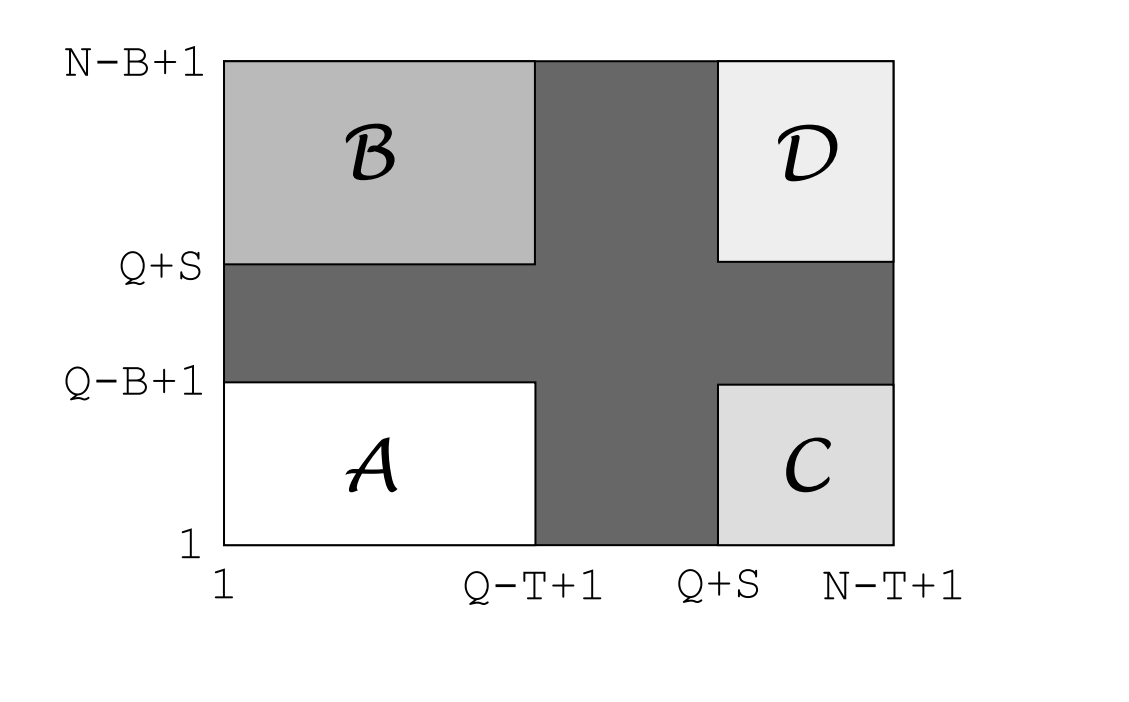
\includegraphics[width=0.7\linewidth]{2.1}}
	\caption{Общая форма матрицы неоднородности.}
	\label{pic:general_form_G}
\end{figure}

\textbf{Крест неоднородности} --- регион в матрице неоднородности с индексами элементов
$$Q-B+1 \leq i \leq Q+S-1, \;\;\; Q-T+1 \leq j \leq Q+S-1.$$
Эти элементы соответствуют тому, что либо тестовый интервал, либо базовый имеет пересечение с переходным.

\newpage
\chapter{Численное сравнение функций разладки}\label{sec:ch_3}

Так как у нас есть четыре функции обнаружения неоднородности:
\begin{enumerate}
	\item 
	Строковая: $d_{n-1}^{(r)} \eqdef h_{b-T}^{(r, 1)} = g(F_{1, B};\; F_{n-T+1, n}), \;\; T \leq n \leq N.$
	
	\item
	Столбцовая: $d_{n-1}^{(c)} \eqdef h_{n-B}^{(1, c)} = g(F_{n-B+1, n};\; F_{1, T}), \;\; B \leq n \leq N.$
	
	\item
	Диагональная: $d_{n-1}^{(d)} \eqdef h_{n-T-B}^{(d, B)} = g(F_{n-T-B+1, n-T+1};\; F_{n-T+1, n}), T + B \leq n \leq N.$
	
	\item
	Симметричная: $d_{n-1}^{(s)} \eqdef h_{n-B}^{(s)} = g(F_{n-B+1, n};\; F_{n-B+1, n}), \;\; B \leq n \leq N.$
	
\end{enumerate}
можем экспериментальным путем попытаться определить, какая из них лучше обнаруживает разладку в ряде.

\section{Постановка задачи}
Рассмотрим ряд $ F_N: F_N = (f_1, \dotsc, f_{N}), N > 2 $, где
\begin{equation}\label{eq:f_n_ch3}
	f_n = 
	\begin{cases}
		C_1\sin(2\pi\omega_1n + \phi_1), & n < Q, \\
		C_2\sin(2\pi\omega_2n + \phi_2), & n \geq Q,
	\end{cases}
\end{equation}
чьи параметры буду задаваться типом разладки и соответствующим изменением параметров.
Рассмотрим два типа неоднородности:
\begin{enumerate}
	\item
	Временную, заданную
	\begin{enumerate}
		\item 
		Фазовым сдвигом: $\phi_1 \neq \phi_2$;
		\item 
		Выбросом:
		$$f_n = 
		\begin{cases}
			C_1\sin(2\pi\omega_1n + \phi_1) & n \neq Q, \\
			10\cdot C_1 & n = Q.
		\end{cases}$$
		\item 
		Изменением амплитуды: $C_1 \neq C_2$.
	\end{enumerate}
	
	\item
	Постоянную, заданную
	\begin{enumerate}
		\item 
		Изменением частоты: $\omega_1 \neq \omega_2$.
	\end{enumerate}
	
\end{enumerate}

Ряды, заданные параметрами выше, порождают матрицы неоднородности, изображенные на Рис. \ref{pic:heterogeneity_types}
\begin{figure}[!hhh]
	\center{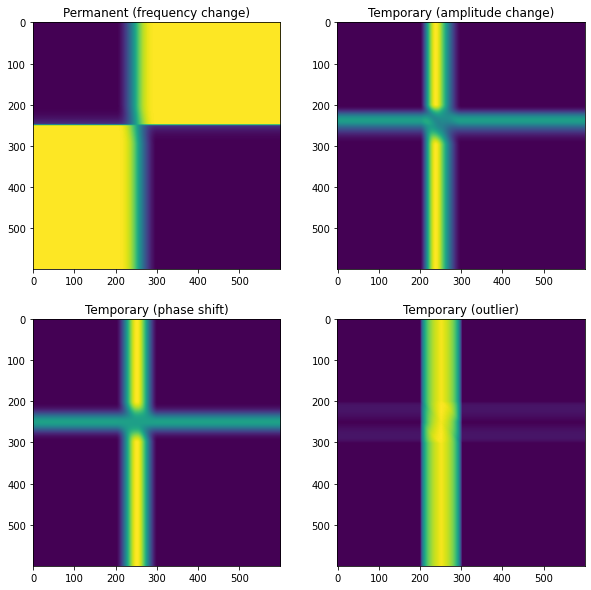
\includegraphics[width=1\linewidth]{heterogeneity_types}}
	\caption{Матрицы неоднородности для рядов без шума.}
	\label{pic:heterogeneity_types}
\end{figure}


В качестве оценок функций неоднородности будем учитывать скорость возрастания значений и момент преодоления $n_{overcome}$ заданного порога $\delta$.


\section{Организация численного эксперимента}
Для реализации тестов был выбран язык $Python3$. Взаимодействие с пакетом $\mathrm{RSSA}$ ~\cite{rssa_package, RSSA_BASIC, RSSA, RSSA_MULTIVATIATE} осуществлялось через библиотеку $rpy2$ (стадии вложения и сингулярного разложения). Подсчет индексов неоднородности велись функционалом языка $Python3$ и библиотеку $numpy$. Работа с графикой велась через библиотеку $matplotlib$. 

Параметры ряда \eqref{eq:f_n_ch3} были заданы следующим образом: 

$ N = 700, \;\omega_1 = \frac{1}{10},\; \omega_2 = \frac{1}{5},\; C_1 = 1, \; C_2 = 2,\; \phi_1=0,\; \phi_2=\frac{\pi}{2},\; Q = 301,\; B = T = 100,\; L = 50,\; r=d=\mathrm{rank}(F_N)=2$.

В тестах предполагаем, что момент разладки $Q$ известен и для оценки скорости возрастания будем выводить значения функций в точках $[Q, Q+10, Q+20, Q+30]$.

Порог, относительно которого будем определять, какая из функций неоднородности раньше обнаруживает разладку, зададим в соответствии с промоделированными значениями, описанными далее.

\newpage

\subsection{Ряды без шума}

Временные ряды и их функции неоднородности изображены на Рис. \ref{pic:TimeSeriesWithoutNoise} и Рис. \ref{pic:HeterFuncsWithoutNoise} соответственно.

Для определения момента преодоления значения порога $ \gamma^* $ необходимо этот порог задать. Для этого к рассмотренным рядам добавим шум $\epsilon\sim N(0, \sigma^2)$, где $\sigma = 0.5$. Для ряда с временной разладкой, заданной изменением амплитуды ($C_1 \neq C_2$), зададим дисперсию шума до разладки как $\frac{\sigma^2}{2}$, чтобы шум $ \epsilon $ был пропорционален амплитуде ряда, так как в противном случае, сила шума не позволит корректно определить базис пространства $ \mathfrak{L_r} $. 

Промоделируем реализации шума $n_{mod}=200$ раз и посчитаем такие характеристики ряда на промежутке $[0, \cdots, Q-1]$, как средний максимум и $95$-й процентиль. Эти два значения возьмем в качестве параметра $ \gamma^* $. 

Результаты моделирования представлены в таблице \ref{tab:ModellingResults}.
\begin{table}[!hhh]
	\center
	\caption{Значения моделирования.}
	\begin{tabular}{lllll}
		Permanent ($\omega_1 \neq \omega_2$) & $ d_{n-1}^{(r)} $ & $ d_{n-1}^{(c)} $ & $ d_{n-1}^{(s)} $ & $ d_{n-1}^{(d)} $ \\
		meanMax & 0.133376 & 0.110945 & 0.130618 & 0.126147 \\
		95 procentile & 0.130877 & 0.110506 & 0.127974 & 0.124446 \\
		&  &  &  &  \\
		Temporary ($C_1 \neq C_2$) & $ d_{n-1}^{(r)} $ & $ d_{n-1}^{(c)} $ & $ d_{n-1}^{(s)} $ & $ d_{n-1}^{(d)} $ \\
		meanMax & 0.036142 & 0.030146 & 0.035325 & 0.034518 \\
		95 procentile & 0.035530 & 0.030024 & 0.034683 & 0.034116 \\
		&  &  &  &  \\
		Temporary ($\phi_1 \neq \phi_2$) & $ d_{n-1}^{(r)} $ & $ d_{n-1}^{(c)} $ & $ d_{n-1}^{(s)} $ & $ d_{n-1}^{(d)} $ \\
		meanMax & 0.132096 & 0.114525 & 0.129501 & 0.124849 \\
		95 procentile & 0.129943 & 0.114098 & 0.127145 & 0.123502 \\
		&  &  &  &  \\
		Temporary (Outlier) & $ d_{n-1}^{(r)} $ & $ d_{n-1}^{(c)} $ & $ d_{n-1}^{(s)} $ & $ d_{n-1}^{(d)} $ \\
		meanMax & 0.132471 & 0.1108 & 0.129573 & 0.127397 \\
		95 procentile & 0.130347 & 0.110320 & 0.127320 & 0.126176
	\end{tabular}
	\label{tab:ModellingResults}
\end{table}


Полученные результаты тестирования функций разладки приведены в таблицах \ref{tab:PermanentHeterogeneity}, \ref{tab:TemporaryHeterogeneityAmplitude}, \ref{tab:TemporaryHeterogeneityShifted}, \ref{tab:TemporaryHeterogeneityOutlier}, а значения функций неоднородности в точках $[Q, Q+10, Q+20, Q+30] $ приведены в таблицах \ref{tab:PermanentHeterogeneityValues}, \ref{tab:TemporaryHeterogeneityAmplitudeValues}, \ref{tab:TemporaryHeterogeneityShiftedValues}, \ref{tab:TemporaryHeterogeneityOutlierValues}.

\begin{figure}[!hhh]
	\center{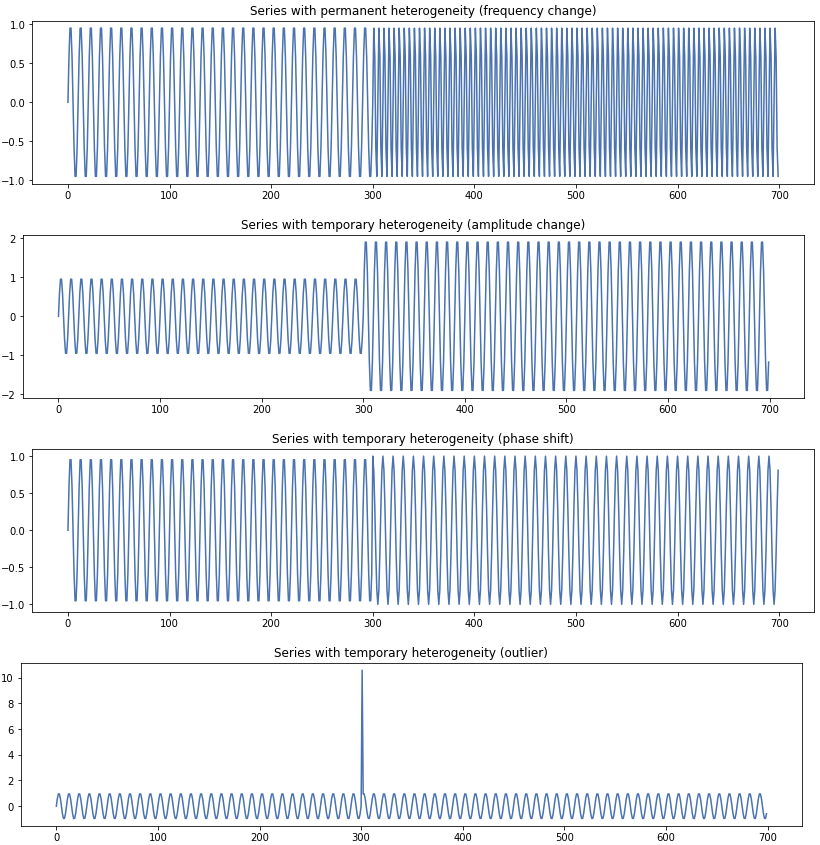
\includegraphics[width=1\linewidth]{seriesTests}}
	\caption{Временные ряды без шума.}
	\label{pic:TimeSeriesWithoutNoise}
\end{figure}

\newpage
\begin{figure}[!hhh]
	\center{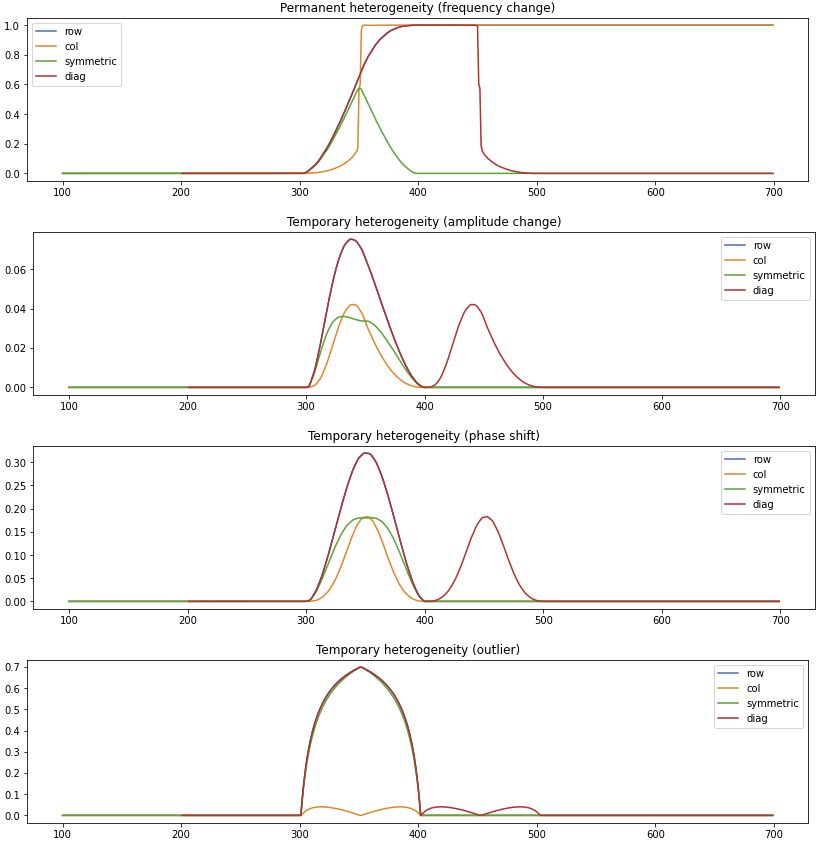
\includegraphics[width=\linewidth]{detectionTests}}
	\caption{Функции неоднородности рядов без шума.}
	\label{pic:HeterFuncsWithoutNoise}
\end{figure}


\newpage
\begin{table}[!hhh]
	\center
	\caption{Характеристики функций неоднородности для постоянной разладки ($\omega_1 \neq \omega_2$).}
	\small
	\begin{tabular}{llllllll}
		Row & 				   & 		  	  & 			 && Col & 		      & 			      \\
		& Statistic        & Mean Max 	  & Mean 95 proc && 	& Mean Max     & Mean 95 proc     \\
		& $n_{overcome}$   & 320   	  & 320      &&     & 345       & 345 		  \\
		&$D_{n_{overcome}}$& 0.134217		  &	0.134217	 &&     & 0.115557		  &   0.115557             \\
		Sym & 				   & 		  	  & 			 && Diag& 		      & 			      \\
		& Statistic        & Mean Max 	  & Mean 95 proc && 	& Mean Max     & Mean 95 proc     \\
		& $n_{overcome}$   & 321   	  & 321      &&     & 320      & 320		  \\
		&$D_{n_{overcome}}$& 0.135379		  &	0.135379		 &&     & 0.134217		 &0.134217                   \\
	\end{tabular}
	\label{tab:PermanentHeterogeneity}
\end{table}

\begin{table}[!hhh]
	\center
	\caption{Значения функций неоднородности в моменты $ [Q, Q+10, Q+20, Q+30] $ при постоянной разладки ($\omega_1 \neq \omega_2$). }
	\begin{tabular}{llllll}
		&              & Row 	  & Col 	& Sym    & Diag  \\
		& $D_Q$        & 0	  & 0 	& 0 & 0		\\
		& $D_{Q+10}$   & 0.042795   & 0.002815  & 0.040179 & 0.042795	\\
		& $D_{Q+20}$   & 0.146766   & 0.013995  & 0.135379 & 0.146766	\\
		& $D_{Q+30}$   & 0.296227	  &	0.038518	& 0.270609 & 0.296227	
	\end{tabular}
	\label{tab:PermanentHeterogeneityValues}
\end{table}

\begin{table}[!hhh]
	\center
	\caption{Характеристики функций неоднородности для временной разладки ($ C_1 \neq C_2 $).}
	\begin{tabular}{llllllll}
		Row & 				   & 		  	  & 			 && Col & 		      & 			      \\
		& Statistic        & Mean Max 	  & Mean 95 proc && 	& Mean Max     & Mean 95 proc     \\
		& $n_{overcome}$   & 317   	  & 317      &&     & 328       & 328 		  \\
		&$D_{n_{overcome}}$& 0.037079		  &	0.037079	 &&     & 0.031576		  &   0.031576             \\
		Sym & 				   & 		  	  & 			 && Diag& 		      & 			      \\
		& Statistic        & Mean Max 	  & Mean 95 proc && 	& Mean Max     & Mean 95 proc     \\
		& $n_{overcome}$   & 327   	  & 326      &&     & 317      & 317		  \\
		&$D_{n_{overcome}}$& 0.035488		  &	0.035066		 &&     & 0.037079		 & 0.037079             \\
	\end{tabular}
	\label{tab:TemporaryHeterogeneityAmplitude}
\end{table}

\begin{table}[!hhh]
	\center
	\caption{Значения функций неоднородности в моменты $ [Q, Q+10, Q+20, Q+30] $ при временной разладки ($ C_1 \neq C_2 $). }
	\begin{tabular}{llllll}
		&              & Row 	  & Col 	& Sym    & Diag  \\
		& $D_Q$        & 0	  & 0 	& 0 & 0		\\
		& $D_{Q+10}$   & 0.018616   & 0.003571  & 0.015156 & 0.018616	\\
		& $D_{Q+20}$   & 0.04911   & 0.018519  & 0.031535 & 0.04911	\\
		& $D_{Q+30}$   & 0.070292	  &	0.036105	& 0.036025 & 0.070292	
	\end{tabular}
	\label{tab:TemporaryHeterogeneityAmplitudeValues}
\end{table}

\newpage

\begin{table}[!hhh]
	\center
	\caption{Характеристики функций неоднородности для временной разладки ($\phi_1 \neq \phi_2$).}
	\begin{tabular}{llllllll}
		Row & 				   & 		  	  & 			 && Col & 		      & 			      \\
		& Statistic        & Mean Max 	  & Mean 95 proc && 	& Mean Max     & Mean 95 proc     \\
		& $n_{overcome}$   & 323   	  & 322      &&     & 336       & 336 		  \\
		&$D_{n_{overcome}}$& 0.140235		  &	0.130778	 &&     & 0.120716		  &   0.120716             \\
		Sym & 				   & 		  	  & 			 && Diag& 		      & 			      \\
		& Statistic        & Mean Max 	  & Mean 95 proc && 	& Mean Max     & Mean 95 proc     \\
		& $n_{overcome}$   & 327   	  & 327      &&     & 322      & 322		  \\
		&$D_{n_{overcome}}$& 0.131381		  &	0.131381		 &&     & 0.130778		 & 0.130778             \\
	\end{tabular}
	\label{tab:TemporaryHeterogeneityShifted}
\end{table}


\begin{table}[!hhh]
	\center
	\caption{Значения функций неоднородности в моменты $ [Q, Q+10, Q+20, Q+30] $ при временной разладки ($\phi_1 \neq \phi_2$). }
	\begin{tabular}{llllll}
		&              & Row 	  & Col 	& Sym    & Diag  \\
		& $D_Q$        & 0.000752	  & 0.000029 	& 0.000723 & 0.000752		\\
		& $D_{Q+10}$   & 0.03919   & 0.00507  & 0.034446 & 0.03919	\\
		& $D_{Q+20}$   & 0.12146   & 0.030249  & 0.096102 & 0.12146	\\
		& $D_{Q+30}$   & 0.21607	  &	0.085474	& 0.150779 & 0.21607	
	\end{tabular}
	\label{tab:TemporaryHeterogeneityShiftedValues}
\end{table}





\begin{table}[!hhh]
	\center
	\caption{Характеристики функций неоднородности для временной разладки (выброс).}
	\begin{tabular}{llllllll}
		Row & 				   & 		  	  & 			 && Col & 		      & 			      \\
		& Statistic        & Mean Max 	  & Mean 95 proc && 	& Mean Max     & Mean 95 proc     \\
		& $n_{overcome}$   & 304   	  & 304      &&     &        &  		  \\
		&$D_{n_{overcome}}$& 0.178852		  &	0.178852	 &&     & 		  &               \\
		Sym & 				   & 		  	  & 			 && Diag& 		      & 			      \\
		& Statistic        & Mean Max 	  & Mean 95 proc && 	& Mean Max     & Mean 95 proc     \\
		& $n_{overcome}$   & 304   	  & 304      &&     & 303      & 303		  \\
		&$D_{n_{overcome}}$& 0.167006		  &	0.167006		 &&     & 0.128127		 & 0.128127             \\
	\end{tabular}
	\label{tab:TemporaryHeterogeneityOutlier}
\end{table}


\begin{table}[!hhh]
	\center
	\caption{Значения функций неоднородности в моменты $ [Q, Q+10, Q+20, Q+30] $ для временной разладки (выброс). }
	\begin{tabular}{llllll}
		&              & Row 	  & Col 	& Sym    & Diag  \\
		& $D_Q$        & 0	  & 0 	& 0 & 0		\\
		& $D_{Q+10}$   & 0.401244   & 0.00357  & 0.380619 & 0.401244	\\
		& $D_{Q+20}$   & 0.546991   & 0.01851  & 0.528819 & 0.546991	\\
		& $D_{Q+30}$   & 0.622343	  &	0.036111 & 0.610083 & 0.622343	
	\end{tabular}
	\label{tab:TemporaryHeterogeneityOutlierValues}
\end{table}

В таблице \ref{tab:TemporaryHeterogeneityOutlier} можно заметить пустые элементы, которые соответствуют ситуациям, когда рассматриваемая функция неоднородности не смогла преодолеть соответствующее промоделированное значение из таблицы \ref{tab:ModellingResults}.

По таблицам \ref{tab:PermanentHeterogeneity}, \ref{tab:TemporaryHeterogeneityAmplitude}, \ref{tab:TemporaryHeterogeneityShifted}, \ref{tab:TemporaryHeterogeneityOutlier} можем сделать вывод, что строковая $d_{n-1}^{(r)}$ и диагональная $d_{n-1}^{(d)}$ функции неоднородности возрастают быстрее остальных, однако $d_{n-1}^{(d)}$ раньше преодолевает промоделированное значение, что значит и более раннее обнаружение разладки.


\newpage
\subsection{Ряды с шумом}
Возьмем те же параметры ряда, что и в предыдущем примере, однако к ряду добавим шум $\epsilon \sim N(0, \sigma^2)$, $\sigma = 0.5$. 

Для ряда с временной разладкой, заданной изменением амплитуды ($C_1 \neq C_2$), зададим дисперсию шума до разладки как $\frac{\sigma^2}{2}$, чтобы шум $\epsilon$ был пропорционален амплитуде ряда, так как в противном случае, сила шума не позволит корректно определить базис пространства $ \mathfrak{L_r} $. 

Для оценки функций неоднородности будем считать порог $ \delta $ как максимум и $ 95 $-й процентиль до момента $ Q $ на каждой итерации.

Временные ряды и их функции неоднородности изображены на Рис. \ref{pic:TimeSeriesWithNoise} и Рис. \ref{pic:HeterFuncsWithNoise} соответственно.

Полученные результаты тестирования функций разладки на рядах с шумом приведены в таблицах \ref{tab:PermanentNoisedHeterogeneity}, \ref{tab:TemporaryHeterogeneityNoisedAmplitude}, \ref{tab:TemporaryHeterogeneityNoisedShifted}, \ref{tab:TemporaryHeterogeneityNoisedOutlier}, а значения функций неоднородности в точках $[Q, Q+10, Q+20, Q+30] $ приведены в таблицах \ref{tab:PermanentNoisedHeterogeneityValues}, \ref{tab:TemporaryHeterogeneityNoisedAmplitudeValues}, \ref{tab:TemporaryHeterogeneityNoisedShifted}, \ref{tab:TemporaryHeterogeneityNoisedOutlierValues}. В данных таблицах приведены средние значения по всем итерациям.

\begin{figure}[!hhh]
	\center{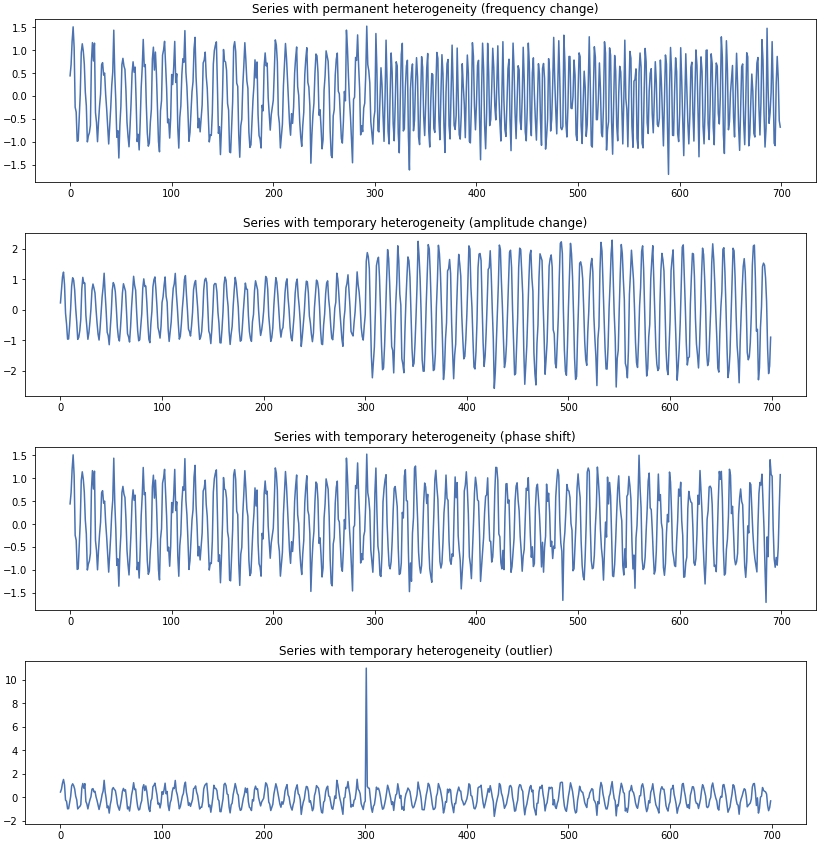
\includegraphics[width=1\linewidth]{seriesNoisedTests}}
	\caption{Временные ряды c шумом.}
	\label{pic:TimeSeriesWithNoise}
\end{figure}

\newpage
\begin{figure}[!hhh]
	\center{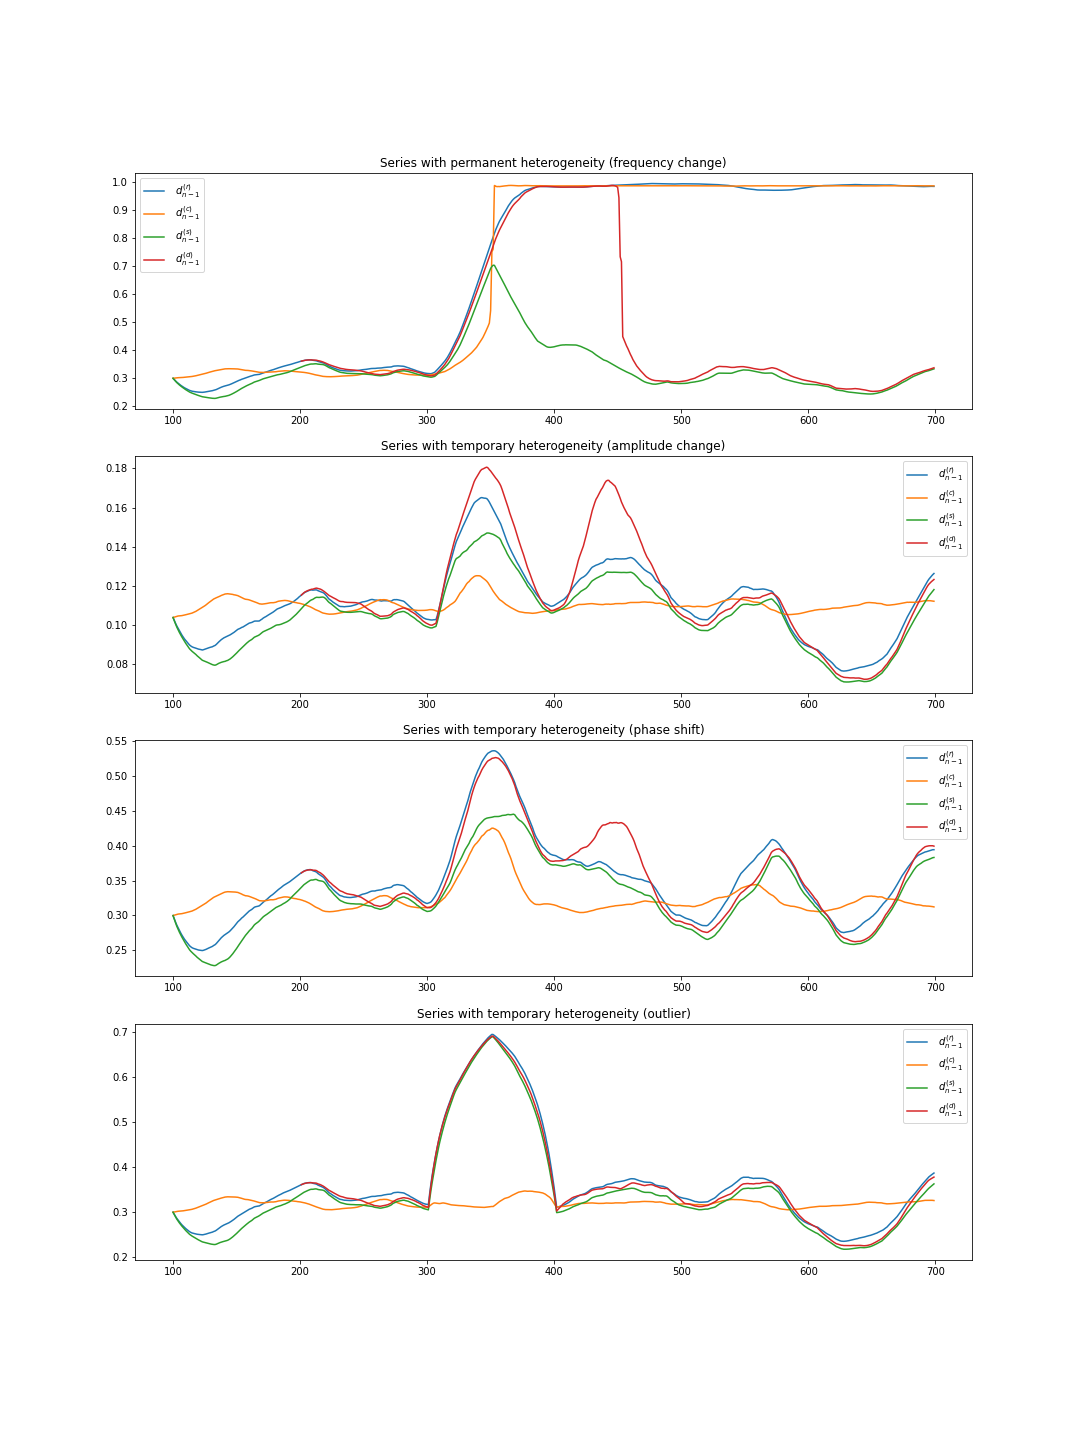
\includegraphics[width=1\linewidth]{detectionNoisedTests}}
	\caption{Функции неоднородности рядов с шумом.}
	\label{pic:HeterFuncsWithNoise}
\end{figure}

\newpage
\begin{table}[!hhh]
	\center
	\small
	\caption{Характеристики функций неоднородности для постоянной разладки ($\omega_1 \neq \omega_2$), с шумом.}
	\begin{tabular}{llllllll}
		Row & 				   & 		  	  & 			 && Col & 		      & 			      \\
		& Statistic        & Mean Max 	  & Mean 95 proc && 	& Mean Max     & Mean 95 proc     \\
		& $\#n_{overcome}$ & 200 	  	  & 200 		 &&     & 200 	      & 200 			  \\
		& $n_{overcome}$   & 309.12   	  & 308.65      &&     & 313,46       & 313,29 		  \\
		& Confidence       & $[309.09, 309.15]$& $[308.61, 308.68]$&&     & $[313.35, 313.57]$ & $[313.17, 313.39]$     \\
		&$D_{n_{overcome}}$& 0.137		  &	0.135		 &&     & 0.1167			  &   0.1165                \\
		Sym & 				   & 		  	  & 			 && Diag& 		      & 			      \\
		& Statistic        & Mean Max 	  & Mean 95 proc && 	& Mean Max     & Mean 95 proc     \\
		& $\#n_{overcome}$ & 200 	  	  & 200 		 &&     & 200 	      & 200 			  \\
		& $n_{overcome}$   & 309.46   	  & 308.94      &&     & 307.78      & 307.45 		  \\
		& Confidence       & $[309.42, 309.49]$ & $[308.91, 308.98]$ &&     & $[307.74, 307.81]$ & $[307.41, 307.48]$     \\
		&$D_{n_{overcome}}$& 0.134		  &	0.131		 &&     & 0.13		 &0,128                   \\
	\end{tabular}
	\label{tab:PermanentNoisedHeterogeneity}
\end{table}

\begin{table}[!hhh]
	\center
	\caption{Значения функций неоднородности в моменты $[Q, Q+10, Q+20, Q+30]$ при разладке, вызванной изменением частот ($\omega_1 \neq \omega_2$) для рядов с шумом}
	\begin{tabular}{llllll}
		&              & Row 	  & Col 	& Sym    & Diag  \\
		& $D_Q$        & 0,1085	  & 0,1075 	& 0,1055 & 0,1084		\\
		& $D_{Q+10}$   & 0,1469   & 0,1102  & 0,1416 & 0,1466	\\
		& $D_{Q+20}$   & 0,2405   & 0,1206  & 0,2273 & 0,2400	\\
		& $D_{Q+30}$   & 0,3734	  &	0,1433	& 0,3476 & 0,3727	
	\end{tabular}
	\label{tab:PermanentNoisedHeterogeneityValues}
\end{table}

\newpage
\begin{table}[!hhh]
	\center
	\small
	\caption{Характеристики функций неоднородности для временной разладки ($С_1 \neq С_2$), с шумом.}
	\begin{tabular}{llllllll}
		Row & 				   & 		  	  & 			 && Col & 		      & 			      \\
		& Statistic        & Mean Max 	  & Mean 95 proc && 	& Mean Max     & Mean 95 proc     \\
		& $\#n_{overcome}$ & 200 	  	  & 200 		 &&     & 200 	      & 200 			  \\
		& $n_{overcome}$   & 306,885   	  & 306,525      &&     & 306,57       & 306,465 		  \\
		& Confidence       & $[306.86, 306.91]$& $[306.50, 306.55]$&&     & $[306.51, 306.63]$ & $[306.41, 306.52]$     \\
		&$D_{n_{overcome}}$& 0,0373		  &	0,0366		 &&     & 0,0321  &   0,032          \\
		Sym & 				   & 		  	  & 			 && Diag& 		      & 			      \\
		& Statistic        & Mean Max 	  & Mean 95 proc && 	& Mean Max     & Mean 95 proc     \\
		& $\#n_{overcome}$ & 200 	  	  & 200 		 &&     & 200 	      & 200 			  \\
		& $n_{overcome}$   & 307,53   	  & 307,07      &&     & 305,94      & 305,745 		  \\
		& Confidence       & $[307.50, 307.56]$ & $[307.04, 307.10]$ &&     & $[305.91, 305.97]$ & $[305.72, 305.77]$     \\
		&$D_{n_{overcome}}$& 0,0363		  &	0,0357		 &&     & 0,0357		 &0,0354          \\
	\end{tabular}
	\label{tab:TemporaryHeterogeneityNoisedAmplitude}
\end{table}

\begin{table}[!hhh]
		\center
		\caption{Значения функций неоднородности в моменты $[Q, Q+10, Q+20, Q+30]$ при разладке, вызванной изменением амплитуд ($ C_1 \neq C_2 $) для рядов с шумом.}
	\begin{tabular}{llllll}
		&              & Row 	  & Col 	& Sym    & Diag  \\
		& $D_Q$        & 0,0296	  & 0,0297 	& 0,0289 & 0,0296		\\
		& $D_{Q+10}$   & 0,0458   & 0,0331  & 0,0418 & 0,0458	\\
		& $D_{Q+20}$   & 0,0713   & 0,0475  & 0,0537 & 0,0713	\\
		& $D_{Q+30}$   & 0,0876	  &	0,0645	& 0,0536 & 0,0873	
	\end{tabular}
	\label{tab:TemporaryHeterogeneityNoisedAmplitudeValues}
\end{table}

\newpage
\begin{table}[!hhh]
	\center
	\caption{Характеристики функций неоднородности для постоянной разладки ($\phi_1 \neq \phi_2$).}
	\small
	\begin{tabular}{llllllll}
		Row & 				   & 		  	  & 			 && Col & 		      & 			      \\
		& Statistic        & Mean Max 	  & Mean 95 proc && 	& Mean Max     & Mean 95 proc     \\
		& $\#n_{overcome}$ & 200 	  	  & 200 		 &&     & 200 	      & 200 			  \\
		& $n_{overcome}$   & 309,37   	  & 308,925      &&     & 311,73       & 311,485 		  \\
		& Confidence       & $[309.33, 309.41]$& $[308.89, 308.96]$&&     & $[311.64, 311.82]$ & $[311.40, 311.57]$     \\
		&$D_{n_{overcome}}$& 0,1351	  &	0,1331		 &&     & 0,1193  &   0,1190         \\
		Sym & 				   & 		  	  & 			 && Diag& 		      & 			      \\
		& Statistic        & Mean Max 	  & Mean 95 proc && 	& Mean Max     & Mean 95 proc     \\
		& $\#n_{overcome}$ & 200 	  	  & 200 		 &&     & 200 	      & 200 			  \\
		& $n_{overcome}$   & 310,105   	  & 309,58      &&     & 307,84      & 307,535 		  \\
		& Confidence       & $[310.06, 310.15]$ & $[309.54, 309.62]$ &&     & $[307.80, 307.88]$ & $[307.50, 307.57]$     \\
		&$D_{n_{overcome}}$& 0,1320		  &	0,1298		 &&     & 0,1282		 &0,1269          \\
	\end{tabular}
	\label{tab:TemporaryHeterogeneityNoisedShifted}
\end{table}

\begin{table}[!hhh]
	\center
	\caption{Значения функций неоднородности в моменты $[Q, Q+10, Q+20, Q+30]$ при разладке, вызванной фазовым сдвигом ($\phi_1 \neq \phi_2$) для рядов с шумом.}
	\begin{tabular}{llllll}
		&              & Row 	  & Col 	& Sym    & Diag  \\
		& $D_Q$        & 0,1078	  & 0,1077 	& 0,1050 & 0,1077		\\
		& $D_{Q+10}$   & 0,1421   & 0,1123  & 0,1351 & 0,1421	\\
		& $D_{Q+20}$   & 0,2158   & 0,1347  & 0,1907 & 0,2158	\\
		& $D_{Q+30}$   & 0,3008	  &	0,1836	& 0,2407 & 0,3005	
	\end{tabular}
	\label{tab:TemporaryHeterogeneityNoisedShiftedValues}
\end{table}

\newpage
\begin{table}[!hhh]
	\center
	\small
	\caption{Характеристики функций неоднородности для временной разладки (выброс), с шумом.}
	\begin{tabular}{llllllll}
		Row & 				   & 		  	  & 			 && Col & 		      & 			      \\
		& Statistic        & Mean Max 	  & Mean 95 proc && 	& Mean Max     & Mean 95 proc     \\
		& $\#n_{overcome}$ & 200 	  	  & 200 		 &&     & 200 	      & 200 			  \\
		& $n_{overcome}$   & 301,935   	  & 301,92      &&     & 303,401       & 303,394		  \\
		& Confidence       & $[301.93, 301.94]$& $[301.916, 301.93]$&&     & $[303.34, 303.46]$ & $[303.33, 303.45]$     \\
		&$D_{n_{overcome}}$& 0,1579	  &	0,1571		 &&     & 0,1185  &   0,1182        \\
		Sym & 				   & 		  	  & 			 && Diag& 		      & 			      \\
		& Statistic        & Mean Max 	  & Mean 95 proc && 	& Mean Max     & Mean 95 proc     \\
		& $\#n_{overcome}$ & 200 	  	  & 200 		 &&     & 200 	      & 200 			  \\
		& $n_{overcome}$   & 301,98   	  & 301,95      &&     & 301,88      & 301,87 		  \\
		& Confidence       & $[301.97, 301.99]$ & $[301.94, 301.96]$ &&     & $[301.86, 301.88]$ & $[301.86, 301.873]$     \\
		&$D_{n_{overcome}}$& 0,1531		  &	0,1517		 &&     & 0,1550		 & 0,1545          \\
	\end{tabular}
	\label{tab:TemporaryHeterogeneityNoisedOutlier}
\end{table}

\begin{table}[!hhh]
	\center
	\caption{Значения функций неоднородности в моменты $[Q, Q+10, Q+20, Q+30]$ при временной разладке  (выброс) для рядов с шумом.}
	\begin{tabular}{llllll}
		&              & Row 	  & Col 	& Sym    & Diag  \\
		& $D_Q$        & 0,1072	  & 0,1100 	& 0,1042 & 0,1071		\\
		& $D_{Q+10}$   & 0,4369   & 0,1423  & 0,5462 & 0,4366	\\
		& $D_{Q+20}$   & 0,5652   & 0,1459  & 0,1907 & 0,5649	\\
		& $D_{Q+30}$   & 0,6336	  &	0,1387	& 0,6204 & 0,6332	
	\end{tabular}
	\label{tab:TemporaryHeterogeneityNoisedOutlierValues}
\end{table}



По результатам видим что в среднем, диагональная функция неоднородности $d_{n-1}^{(d)}$ раньше обнаруживает разладку среди остальных трех, при этом, уступая в скорости возрастания строковой в примерах с постоянной ($\omega_1 \neq \omega_2$) и временной (выброс) разладками. 

\newpage
\section{Выводы}

\begin{table}[!hhh]
	\center
	\caption{Средние значения характеристик функций обнаружения по всем типам неоднородности.}
	\begin{tabular}{lllllll}
		Row & meanMax & 95 procentile \\
		$\#n_{overcome}$ & 200 & 200 \\
		$n_{overcome}$ & 306.83 & 306.5 \\
		$||[D_Q^{(r)},\; D_{Q+10}^{(r)},\; D_{Q+20}^{(r)},\; D_{Q+30}^{(r)}]||_{L_2})$ & 0.49439 &  \\
		&  &  \\
		Col & meanMax & 95 procentile \\
		$\#n_{overcome}$ & 199.25 & 199.5 \\
		$n_{overcome}$ & 308.79 & 308.66 \\
		$||[D_Q^{(c)},\; D_{Q+10}^{(c)},\; D_{Q+20}^{(c)},\; D_{Q+30}^{(c)}]||_{L_2}$ & 0.2199 & \\
		&  &  \\
		Sym & meanMax & 95 procentile \\
		$\#n_{overcome}$ & 200 & 200 \\
		$n_{overcome}$ & 307.27 & 306.89 \\
		$||[D_Q^{(s)},\; D_{Q+10}^{(s)},\; D_{Q+20}^{(s)},\; D_{Q+30}^{(s)}]||_{L_2}$ & 0.45628 & \\
		&  &  \\
		Diag & meanMax & 95 procentile \\
		$\#n_{overcome}$ & 200 & 200 \\
		$n_{overcome}$ & 305.86 & 305.65 \\
		$||[D_Q^{(d)},\; D_{Q+10}^{(d)},\; D_{Q+20}^{(d)},\; D_{Q+30}^{(d)}]||_{L_2}$ & 0.49389 & 
	\end{tabular}
	\label{tab:AvgResultsNoise}
\end{table}

Явными фаворитами (таблица \ref{tab:AvgResultsNoise}) являются строковая $d_{n}^{(r)}$ и диагональная $d_{n}^{(d)}$ функции неоднородности. Они обе показывают превосходство над столбцовой $d_{n}^{(c)}$ и симметричной $d_{n}^{(s)}$ в устойчивости к шуму $\epsilon$, моментом обнаружения разладки $n_{overcome}$ и скорости возрастания значений $[D_Q, D_{Q+10}, D_{Q+20}, D_{Q+30}]$ после момента нарушения однородности $Q$.


\newpage
\chapter{Аналитическая оценка индекса неоднородности при изменении частоты гармоники} \label{sec:ch_4}
В качестве функции неоднородности будем рассматривать строковую $ d_n $.

Рассмотрим ряд $ F_N = (f_1, \dots f_{N}) $, причем  
\begin{equation*} 
	f_n = 
	\begin{cases} 
		C_1\sin(2\pi\omega_1 n + \phi_1),\ n \in [1, Q-1] \\ 
		C_2\sin(2\pi\omega_2 n + \phi_2),\ n \in [Q, N] 
	\end{cases} 
\end{equation*} 

Обозначим 
$$ F^{(1)} = f_n^{(1)}|_{n=1}^{B}, $$
$$ F^{(2)} = f_n^{(2)}|_{n=1}^{T}, $$
$$X_l^{(2)} = (f_{l}^{(2)}, \dotsc, f_{l+L-1}^{(2)})^\mathrm{T}, \;\;\; 1 \leq l < K_2.$$

В обозначениях выше, $ F^{(1)} $ --- некий подряд ряда $ F_N $ длины $ B $, целиком лежащий в промежутке от начала ряда до точки разладки $ Q $, а  $ F^{(2)} $ --- некий подряд ряда $ F_N $ длины $ T $, целиком лежащий в промежутке от точки разладки $ Q $ до конца ряда $ F_N $. 


В соответствии с формулой \eqref{eq:g}, индекс неоднородности задается как:
$$ g(F^{(1)}; F^{(2)}) = 1 - \frac{\sum\limits_{l=0}^{K_2-1}\;\sum\limits_{i=0}^{r-1}\langle X_l^{(2)}, U_i^{(1)}\rangle^2}{\sum\limits_{l=0}^{K_2-1}\|X_l^{(2)}\|^2} = 1 - z(F^{(1)}; F^{(2)}),  $$
где $ z(F^{(1)}; F^{(2)}) $ --- индекс однородности.

В данной главе будем предполагать $ \omega_1 \neq \omega_2;\; C_1 = C_2 $. Для простоты зададим амплитуды $ C_1 = C_2 = 1 $.

Попробуем аналитически упростить данную формулу, чтобы явно увидеть, как разности частот ряда до и после разладки влияют на значения $ g $.

\section{Аппроксимация индекса однородности}
Рассмотрим индекс однородности $ z $ при $ N \rightarrow \infty $, $ T \rightarrow \infty $, $ L \rightarrow \infty $. Поскольку $ K_2 = T - L + 1 \Rightarrow K_2 \rightarrow \infty $.


\subsection{Знаменатель}
Начнем со знаменателя $\sum\limits_{l=1}^{K_2}\|X_l^{(2)}\|^2$, а точнее, с квадрата нормы $\|X_l^{(2)}\|^2$. Оценим его:

$$ \|X_l^{(2)}\|^2 = \sum\limits_{i=1}^{L}(X_{l}^{(2)})_i^2 \approx \int\limits_{0}^{L}\sin^2{(2\pi\omega_2 y + \psi_l)}dy = \frac{L}{2} - \frac{\sin(4\pi L\omega_2 + \psi_l) - \sin(2\psi_l)}{8\pi\omega_2} \approx \frac{L}{2}, $$
где $ \psi_l $ формируется из $ \phi_2 $ и сдвига, порождаемого номером вектора вложения.

Отсюда $\sum\limits_{l=1}^{K_2}\|X_l^{(2)}\|^2 \approx K_2\cdot\frac{L}{2}$.


\subsection{Числитель}
$$ \sum\limits_{l=1}^{K_2}\;\sum\limits_{i=1}^{r}\langle X_l^{(2)}, U_i^{(1)}\rangle^2 = 
\sum\limits_{l=1}^{K_2}\;\left ( \langle X_l^{(2)}, U_1^{(1)}\rangle^2 + \langle X_l^{(2)}, U_2^{(1)}\rangle^2 \right ) = $$
$$ =  \sum\limits_{l=1}^{K_2}\; \left [ \left (\sum\limits_{j=1}^{L}(X_{l}^{(2)})_j\cdot (U_{1}^{(1)})_j\right )^2 + \left ( \sum\limits_{j=1}^{L}(X_{l}^{(2)})_j\cdot (U_{2}^{(1)})_j\right )^2 \right ].$$

Рассмотрим $ U_{1}^{(1)} $ и $U_{2}^{(1)} $. В силу задания ряда, при условии $ L\omega_1 $ --- целое число, ортонормированным базисом $ U_{1}^{(1)} $ и $U_{2}^{(1)} $ пространства $ \mathfrak{L}_r^{(1)} $, порожденного элементами $ f_n^{(1)} = \sin(2\pi\omega_1 n + \phi_1) $ являются $ \sin(2\pi\omega_1 n) $ и $ \cos(2\pi\omega_1 n) $. Если $ L\omega_1 $ целым не является, будем считать что эти элементы приближенно ортонормированы.

Пусть $ P_1 = \{\sin(2\pi\omega_1 n)\}_{n=1}^L $, $ P_2 = \{\cos(2\pi\omega_1 n)\}_{n=1}^L $. Вычислим нормы $ P_1 $ и $ P_2 $ для поиска $ U_{1}^{(1)} $ и $U_{2}^{(1)} $. 
По аналогии со знаменателем индекса однородности (п. 5.1.1.), $ \|p_1\| = \|p_2\| \approx \sqrt{\frac{L}{2}} $, откуда $ U_{1}^{(1)} = \frac{\sin(2\pi\omega_1 n)}{\sqrt{L/2}} $, $ U_{2}^{(1)} = \frac{\cos(2\pi\omega_1 n)}{\sqrt{L/2}} $.

Пусть  
$$ I_l =  \left (\sum\limits_{j=1}^{L}(X_{l}^{(2)})_j\cdot (U_{1}^{(1)})_j\right )^2, $$
$$ J_l =  \left (\sum\limits_{j=1}^{L}(X_{l}^{(2)})_j\cdot (U_{2}^{(1)})_j\right )^2, $$
$$ a = \omega_1 + \omega_2,\ b = \omega_1 - \omega_2. $$

Тогда
$$ I_l \approx \left( \int\limits_{0}^{L}\sin(2\pi\omega_2 y + \psi_l) \cdot \frac{\sin(2\pi\omega_1 y)}{\sqrt{L/2}}dy \right)^2 = $$
$$ = \frac{2}{L} \left(\int\limits_{0}^{L}\sin(2\pi\omega_2 y) \cdot \sin(2\pi\omega_1 y)dy\right )^2 = $$
$$ = \frac{2}{L} 
\left(  
\frac{\sin(2\pi Lb - \psi_l) + \sin(\psi_l)}{4\pi b} - \frac{\sin(2\pi La + \psi_l) - \sin(\psi_l)}{4\pi a}
\right)^2. $$



$$ J_l \approx \left(\int\limits_{0}^{L}(\sin(2\pi\omega_2 y + \psi_l) \cdot \frac{\cos(2\pi\omega_1 y)}{\sqrt{L/2}})dy\right)^2 = $$
$$ = \frac{2}{L}\left(\int\limits_{0}^{L}(\sin(2\pi\omega_2 y + \psi_l) \cdot\cos(2\pi\omega_1 y))dy\right )^2 = $$
$$ = \frac{2}{L} 
\left(  
\frac{\cos(2\pi Lb - \psi_l) - \cos(\psi_l)}{4\pi b} - \frac{\cos(2\pi La + \psi_l) - \cos(\psi_l)}{4\pi a}
\right)^2. $$


Так как $ \psi_l $ формируются из сдвига, порождаемого номером вектора вложения, а исходный ряд $ F_N $ задан синусом, при суммировании и достаточно большом значении $ K_2 $, сумма по периоду асимптотически обращается в $ 0 $, поэтому при переходе к сумме по элементам $ X_l^{(2)}, l=1, \dots, K_2 $, зависимость от $ \psi_l $ пропадает.

Обозначим
$$ I = \frac{2}{L} \left(  \frac{\sin(2\pi Lb)}{4\pi b} - \frac{\sin(2\pi La)}{4\pi a}   \right)^2. $$
$$ J = \frac{2}{L} \left(  \frac{\cos(2\pi Lb) - 1}{4\pi b} - \frac{\cos(2\pi La) - 1}{4\pi a}  \right)^2. $$


С учетом предположения выше, получаем:

$$ \sum\limits_{l=1}^{K_2}\;\sum\limits_{i=1}^{r}\langle X_l^{(2)}, U_i^{(1)}\rangle^2 \approx K_2 \cdot \left [ I_l + J_l \right] = $$
$$ = \frac{K_2 \cdot 2}{L} \cdot \left[ \left(  \frac{\sin(2\pi Lb)}{4\pi b} - \frac{\sin(2\pi La)}{4\pi a}   \right)^2 + \left(  \frac{\cos(2\pi Lb) - 1}{4\pi b} - \frac{\cos(2\pi La) - 1}{4\pi a}  \right)^2 \right] $$


\section{Индекс неоднородности}
Собирая все вместе, получаем:

$$ g(F^{(1)}; F^{(2)}) = 1 - \frac{\sum\limits_{l=0}^{K_2-1}\;\sum\limits_{i=0}^{r-1}\langle X_l^{(2)}, U_i^{(1)}\rangle^2}{\sum\limits_{l=0}^{K_2-1}\|X_l^{(2)}\|^2} \approx $$
$$ \approx 1 - \frac{\frac{K_2 \cdot 2}{L} \cdot \left[ \left(  \frac{\sin(2\pi Lb)}{4\pi b} - \frac{\sin(2\pi La)}{4\pi a}   \right)^2 + \left(  \frac{\cos(2\pi Lb) - 1}{4\pi b} - \frac{\cos(2\pi La) - 1}{4\pi a}  \right)^2 \right]}{K_2\cdot\frac{L}{2}} = $$
\begin{equation}\label{eq:g_a}
	= 1 - \frac{\left[ \left(  \frac{\sin(2\pi Lb)}{4\pi b} - \frac{\sin(2\pi La)}{4\pi a}   \right)^2 + \left(  \frac{\cos(2\pi Lb) - 1}{4\pi b} - \frac{\cos(2\pi La) - 1}{4\pi a}  \right)^2 \right]}{\frac{L^2}{4}} = g_a(\omega_1, \omega_2).
\end{equation}


\section{Проверка точности аппроксимации}
При сравнении индекса неоднородности, вычисленного классическим способом и аналитически упрощенным, результаты оказались довольно похожи, причем при $L \rightarrow \infty $ оба значения сходятся друг к другу. Все тесты доступны в гитхаб репозитории~\cite{github} в файле \textbf{Analytical.ipynb}.



\subsection{Одинаковые частоты}
Пусть $ N = 700,\; Q = 301,\; B = 100,\; T = 100 $. 
Зададим $\omega_1 = \frac{1}{10},\; \omega_2 = \frac{1}{10},\; L = 60$. При одинаковых частотах значения индексов неоднородности должны быть равны $ 0 $. Действительно, по определению $ g $ пространство $ \mathfrak{L}_r $, порожденное рядом $ F_N $ является одним и тем же для любых подрядов $ F^{(1)} $ и $ F^{(2)} $ ряда $ F_N $ так как структура ряда не менялась.
Проверяя этот теоретический факт численно, получили также $ 0 $.

\subsection{$L\omega_1$ и $L\omega_2 $ целые, $\omega_1 \neq \omega_2 $}
Еще один теоретический факт: 

При целых $L\omega_1$ и $L\omega_2 $ индекс однородности $ z $ обращается в 0. Действительно, в силу построения ряда (гармоника, описываемая синусом с какими-то фиксированными параметрами), скалярное произведение частей исходного ряда по целому периоду на элементы базиса (ортогональные друг другу) обращают числитель в 0, следовательно индекс неоднородности $ g $ всегда равен $ 1 $, что подтверждено численно.


\subsection{Зависимость от $ L $}

Зафиксируем $ \omega_2 $ и будем изменять $ L $. 

Чтобы наглядно продемонстрировать стремление значений друг к другу, посмотрим на Рис. \ref{pic:g_c_vs_g_a_from_L} и \ref{pic:g_c_vs_g_a_from_L_1}.

\begin{figure}[!hhh]
	\center{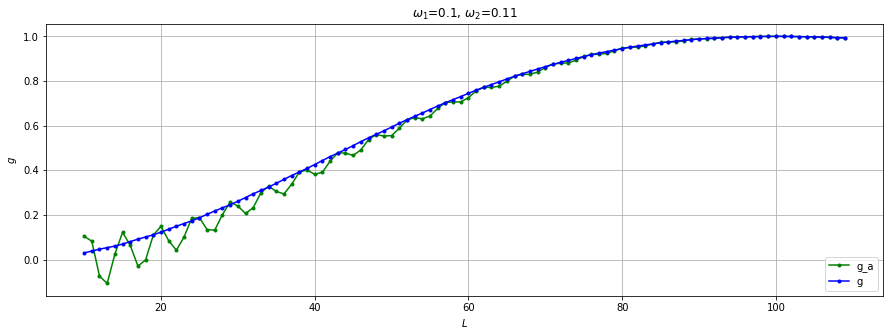
\includegraphics[width=1.0\linewidth]{dynamics_L}}
	\caption{Зависимость индексов $ g $ и $ g_a $ от $ L $ при $ \omega_2 = 0.11 $.}
	\label{pic:g_c_vs_g_a_from_L}
\end{figure}

\begin{figure}[!hhh]
	\center{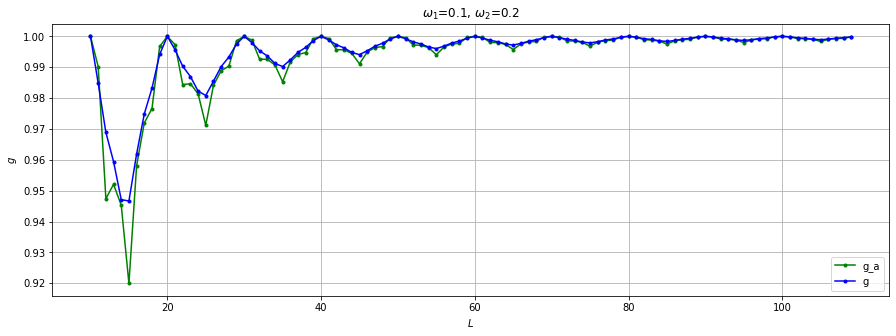
\includegraphics[width=1.0\linewidth]{dynamics_L_1}}
	\caption{Зависимость индексов $ g $ и $ g_a $ от $ L $ при $ \omega_2 = 0.2 $.}
	\label{pic:g_c_vs_g_a_from_L_1}
\end{figure}



Исходя из кривых на Рис. \ref{pic:g_c_vs_g_a_from_L} и \ref{pic:g_c_vs_g_a_from_L_1}, $ g \rightarrow 1 \text{ при } L \rightarrow \infty$ --- справедливо для обеих формул \eqref{eq:g}, \eqref{eq:g_a}. 

Данный эксперименты подтверждает что при достаточно больших $ L $ аппроксимация индекса неоднородности выведенной аналитической формулой \eqref{eq:g_a} точна.

\subsection{Зависимость от разности $\omega_1$ и $ \omega_2 $}
\newtheorem{statement}{Утверждение}

Покажем, что чем больше разница между $ \omega_1 $ и $ \omega_2 $, тем проще определить разладку.

Иными словами, чем больше разница $ \omega_1 $ и $ \omega_2 $, тем быстрее индекс неоднородности $ g $ переходит в $ 1 $.

Пусть $ \omega_1 \geq \omega_2, \; \omega_2 \rightarrow \omega_1 $. Аналитически, в пределе $ a = 2\omega_1,\; b = 0 $. Тогда формула \eqref{eq:g_a} примет вид 
$$ g_a(\omega_1, \omega_2) \approx g_a(\omega_1, \omega_1) = 1 - \frac{(\frac{L}{2} - \frac{\sin(4\pi L\omega_1)}{8\pi\omega_1} + \frac{\omega_1}{2\pi\omega_1^2})^2}{\frac{L^2}{4}} \approx 1 - \frac{(\frac{L}{2})^2}{\frac{L^2}{4}} = 1 - 1 = 0 $$

При численной проверке, получились значения $ g = 0.0,\; g_a = 3.330669e-16 \approx 0 $.

Посмотрим на график зависимости $ g $ от $ \omega_2 $ при фиксированном $ \omega_1 = \frac{1}{10} $.

\begin{figure}[!hhh]
	\center{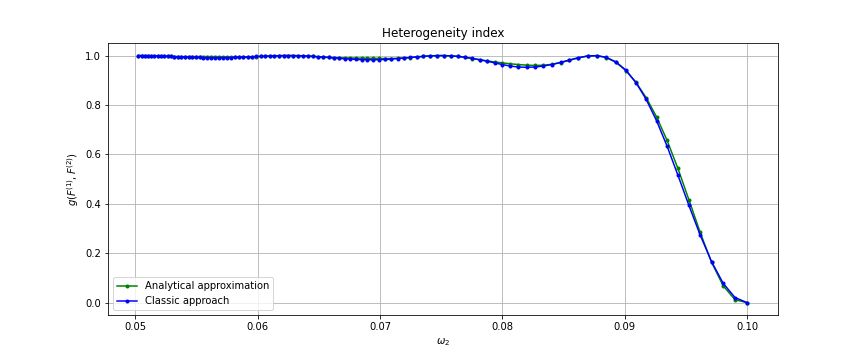
\includegraphics[width=1.0\linewidth]{dynamics_w2}}
	\caption{Зависимость индексов $ g $ и $ g_a $ от $ \omega_2 $.}
	\label{pic:g_c_vs_g_a_from_w_2}
\end{figure}

По кривым на Рис. \ref{pic:g_c_vs_g_a_from_w_2} видим, что чем ближе частоты друг к другу, тем ближе индекс неоднородности к $ 0 $, и, соответственно, чем дальше, тем ближе $ g $ к $ 1 $.


\newpage
\chapter{Система обнаружения структурной неоднородности ряда с автоматически выстраиваемым порогом срабатывания} \label{sec:ch_5}

В данной главе будет рассматриваться только строковая функция обнаружения неоднородности $ d_n^{(r)} $, обозначим ее как $ d_n $.


Рассмотрим ряд $ F_N = (f_1, \dots f_{N}) $, причем  
\begin{equation*} 
	f_n = 
	\begin{cases} 
		C\sin(2\pi\omega_1 n + \phi_1),\ n \in [1, Q-1] \\ 
		C\sin(2\pi\omega_2 n + \phi_2),\ n \in [Q, N], 
	\end{cases} 
\end{equation*} 
где $ Q $ --- момент возмущения. 

Обозначим
$$ F^{(1)} = f_n^{(1)}|_{n=1}^{B}, $$
$$ F^{(2)} = f_n^{(2)}|_{n=1}^{T}, $$
$$ X_l = (f_{l}^{(2)}, \dotsc, f_{l+L-1}^{(2)})^\mathrm{T}, \;\;\; 1 \leq l < K_2. $$

Рассмотрим систему, которая получает на вход ряд $ F_N $ и порог $ \gamma^* $.

\begin{algorithm}\label{algo:system_works}
	Описание системы:
	\begin{enumerate}
		\item Входные данные: $ F_N $, $ \gamma^* \in \mathbb{R}_{[0, 1]} $;
		\item Результат: $\hat{Q}$ --- момент преодоления $ d_n $ значения $ \gamma $;
		\end{enumerate}
\end{algorithm}

Введем требование к системе --- $ \hat{Q} \in [Q, Q+k] $, где параметр $ k \in \mathbb{N} $ --- максимальное запаздывание для обнаружения неоднородности, полученный из входных данных. 

Поскольку подача на вход значения $ \gamma^* $ никак не зависит от $ k $, будем выбирать порог алгоритмически. Таким образом, основная задача состоит в нахождении порога. 
\begin{algorithm}\label{algo:fix_gamma}
	Нахождение порога $ \gamma^* $:
	\begin{enumerate}
		\item Построить функцию $ \gamma: \mathbb{N} \rightarrow [0, 1] $, аппроксимирующую поведение функции $ d_n $ после момента $ Q $.
		\item Брать $ \gamma^* $ как значение функции $ \gamma $ в точке $ k $.
	\end{enumerate}
\end{algorithm}

Для построения $ \gamma $, сначала рассмотрим нижнюю и верхнюю границы $ \gamma^* $, которые зависят от значения функции $ d_n $ до переходного интервала и после.

\section{Оценка $ \gamma^* $}
\subsection{Нижняя граница}\label{ch:lower_border}

При наличии шума $ \epsilon $ с дисперсией $ \sigma^2 $, значения $ d_n $ до момента $ Q $ смещаются от $ 0 $ вверх примерно на $ \frac{\sigma^2}{C^2/2 + \sigma^2} $ (Рис. \ref{pic:estimate_gamma_lower}). Если взять нижнюю границу $ \gamma^* $ слишком маленьким, то $ \hat{Q} < Q $, произойдет ложное срабатывания системы. Пусть нижняя граница $ \gamma_{min} $ задается как
\begin{equation}\label{eq:gamma_min}
	\gamma_{min}(\sigma^2) = \frac{\sigma^2}{C^2/2 + \sigma^2}
\end{equation}

\begin{figure}[!hhh]
	\center{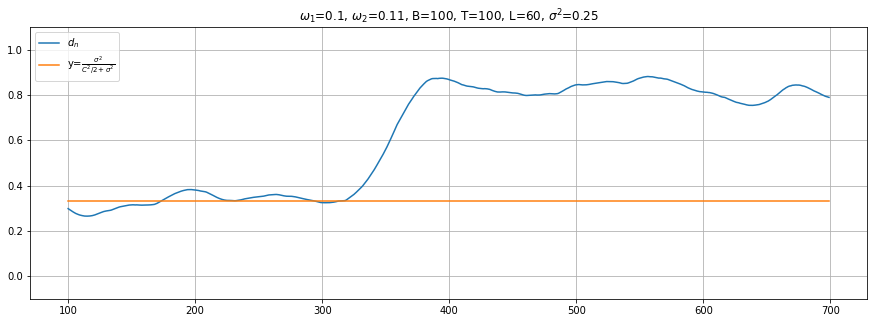
\includegraphics[width=1.0\linewidth]{estimate_gamma_lower.png}}
	\caption{Оценка $ \gamma^* $. Нижняя граница.}
	\label{pic:estimate_gamma_lower}
\end{figure}

\subsection{Верхняя граница}\label{ch:apper_border}
В качестве верхней границы $ \gamma^* $ будет выступать значение функции $ \gamma $ в точке $ k $. Для построения $ \gamma $, нам надо знать значение $ d_n $ после переходного интервала, для вычисления которого мы можем воспользоваться аналитической аппроксимацией индекса неоднородности $ g_a(\omega_1, \omega_2) $ по формуле \eqref{eq:g_a}, однако нам нужно знать частоты до и после разладки.

Поведение функции неоднородности $ d_n $ на переходном отрезке зависит от значения после переходного отрезка. По свойству индекса неоднородности, чем больше $ |\omega_2 - \omega_1| $, тем ближе $ g $ к $ 1 $ после переходного интервала, следовательно, кривая $ d_n $ на переходном интервале будет иметь более крутой наклон (Рис. \ref{pic:diff_omega_growth}).

\begin{figure}[!hhh]
	\center{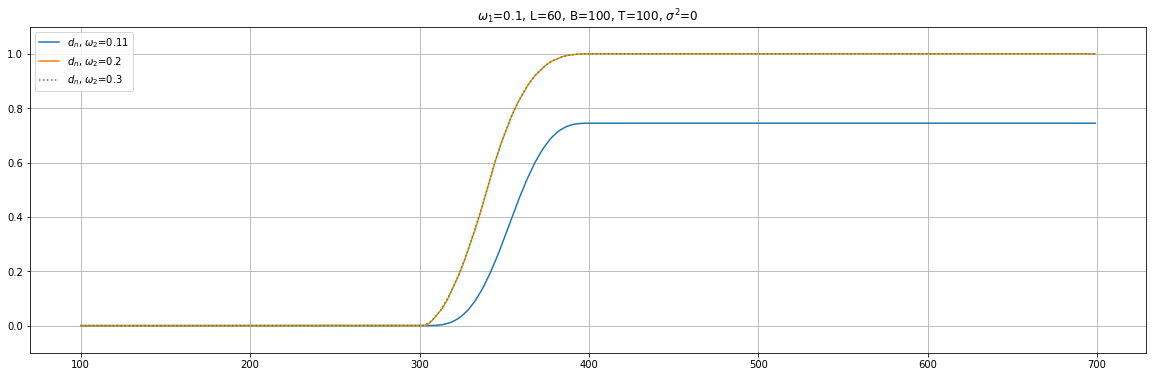
\includegraphics[width=1.0\linewidth]{diff_omega_growth.png}}
	\caption{Оценка $ \gamma^* $. Скорость возрастания $ d_n $ на переходном интервале.}
	\label{pic:diff_omega_growth}
\end{figure}

Добавим еще $ 2 $ параметра, подаваемых на вход системе:
\begin{enumerate}
	\item $ \omega_1 $ --- начальная частота ряда;
	\item $ \Delta_{min} $ --- минимальное по модулю отклонение частоты ряда от $ \omega_1 $ для обнаружения неоднородности.
\end{enumerate}

Обозначим $ \omega_{min} = \omega_1 + \Delta_{min}$. Численно проверено, что $ g_a(\omega_1, \omega_1 + \Delta_{min}) \approx g_a(\omega_1, \omega_1 - \Delta_{min}) $ при достаточно большом значении $ L $.

Таким образом, имея значение $ g_a(\omega_1, \omega_{min}) $, мы можем вычислить $ \gamma^* $ как значение аппроксимации переходного интервала $ \gamma(i), i=1, \dots, T $ кривой $ d_n, n=Q, \dots, Q+T, $ в точке $ k $, которая соединяет $ \gamma_{min} $ и $ g_a(\omega_1, \omega_{min}) $. 

Введем еще одно обозначение для наглядности дальнейших результатов исследования. Так как $ \gamma $ --- аппроксимация переходного интервала функции $ d_n $, введем $ a_n $ --- аппроксимацию всей кривой $ d_n $.
\begin{equation}\label{eq:a_n}
	a_n = 
	\begin{cases}
		\gamma_{min}, n < Q,\\
		\gamma(n), n \in [Q, Q+T],\\
		g_a(\omega_1, \omega_{min}), n > Q.
	\end{cases}
\end{equation}


\section{Аппроксимация переходного интервала}\label{ch:approx_d_n}
Рассмотрим траекторные матрицы $ \mathbb{X}_{test}^{(j)} $ размерности $ L \times K_{test} $ тестовых рядов $ F_N^{(2)} = F_{j, j+T} $, где $ K_{test} = T - L + 1 $, $ j \in [0, N-T) $. 

$ \forall \; j \in [0, Q - T), \forall \; n \in [1, K_{test}]: $ для $ n $-го столбца матрицы $ \mathbb{X}_{test}^{(j)},  \mathrm{X}_n \in \mathfrak{L}_r^{(1)} $. 

$ \forall \; j \in [Q+T, N-T), \forall \; n \in [1, K_{test}]: $ для $ n $-го столбца матрицы $ \mathbb{X}_{test}^{(j)},  \mathrm{X}_n \notin \mathfrak{L}_r^{(1)} $. 

\bigskip

При $ T > 2 \cdot L $, $ \forall \; j \in [Q - T + L, Q - L)$, $ \mathbb{X}_{test}^{(j)} $ состоит из:

\begin{itemize}
	\item $ n_B = n_B(j) $ векторов вложений, лежащих в $ \mathfrak{L}_r^{(1)} $;
	\item $ n_Q = n_Q(j) $ векторов вложений, содержащих момент возмущения;
	\item $ n_A = n_A(j) $ векторов вложений, содержащих только значения ряда после разладки.
\end{itemize}

Причем $ K_{test} = n_B + n_Q + n_A $

Пусть $ L $ --- фиксировано. 

$$ g(F^{(1)}; F^{(2)}) = \frac{\sum\limits_{l=1}^{K_{test}}\mathrm{dist}^2(X_l, \mathfrak{L}_r^{(1)})}{\sum\limits_{l=1}^{K_{test}}\|X_l\|^2} = $$
$$ = \frac{\sum\limits_{l=1}^{n_B}\mathrm{dist}^2(X_l, \mathfrak{L}_r^{(1)}) + \sum\limits_{l=n_B}^{n_B + n_Q}\;\mathrm{dist}^2(X_l, \mathfrak{L}_r^{(1)}) + \sum\limits_{l=n_B + n_Q}^{K_{test}}\;\mathrm{dist}^2(X_l, \mathfrak{L}_r^{(1)})}{\sum\limits_{l=1}^{n_B}\|X_l\|^2 + \sum\limits_{l=n_B}^{n_B+n_Q}\|X_l\|^2 + \sum\limits_{l=n_B+n_Q}^{K_{test}}\|X_l\|^2} \approx $$
\begin{equation}\label{eq:linear_g}
	\approx \frac{0 + \sum\limits_{l=n_B}^{n_B+n_Q}\;\mathrm{dist}^2(X_l, \mathfrak{L}_r^{(1)}) + n_A(j) \cdot c_H}{K_{test}\cdot \frac{L}{2}} \approx \frac{n_A(j) \cdot c_H}{K_{test}\cdot \frac{L}{2}},
\end{equation}

при $ T \rightarrow \infty $ в силу $ n_Q = o(T) $.

Так как для вычисления $ d_n $ мы последовательно смещаем тестовые ряды на $ 1 $ элемент, $ n_A(j) $ возрастает линейно, начиная c $ j = Q-T+L $, $ n_A(j) = j - Q + T - L $. Получили в правой части формулы \eqref{eq:linear_g} линейную функцию. 

Действительно, при увеличении $ T $ --- увеличивается количество $ K_{test} $ элементов, что приводит к увеличению $ n_B $ и $ n_A $, и уменьшению вклада каждого $ \mathrm{X}_l $ в $ g $. Так как $ \forall j \; n_Q(j) \leq L $ при $ T \rightarrow \infty $ вклад соответствующих $ \mathrm{X}_l $ в $ g $ пренебрежительно мал.

Аналогичная ситуация и при уменьшении $ L $. Таким образом, чем больше разность $ T-L $, тем линейнее переходный интервал кривой $ d_n $ (Рис. \ref{pic:row_linear_growth}).


\begin{figure}[!hhh]
	\center{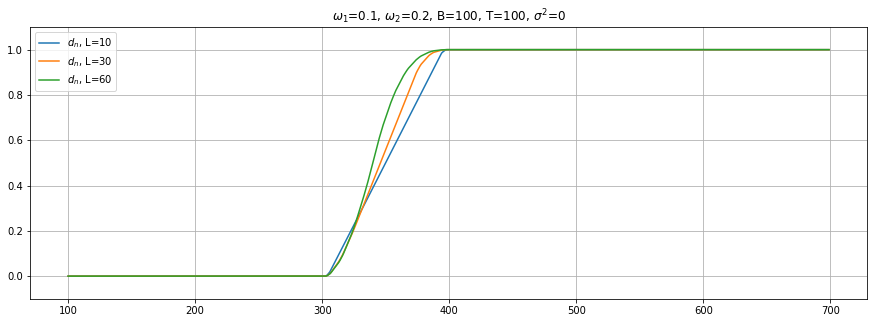
\includegraphics[width=1.0\linewidth]{row_linear_growth.png}}
	\caption{Аппроксимация переходного интервала. Линейность при увеличении разности $ T-L $.}
	\label{pic:row_linear_growth}
\end{figure}


Таким образом, мы можем аппроксимировать переходный интервал кривой $ d_n $ от $ \gamma_{min} $ до $ g_a(\omega_1, \omega_{min}) $ линейной функцией $ \gamma(i),\; i=1, \dots, T $ (Рис. \ref{pic:row_linear_approximation_1}, \ref{pic:row_linear_approximation_2}).

\begin{figure}[!hhh]
	\center{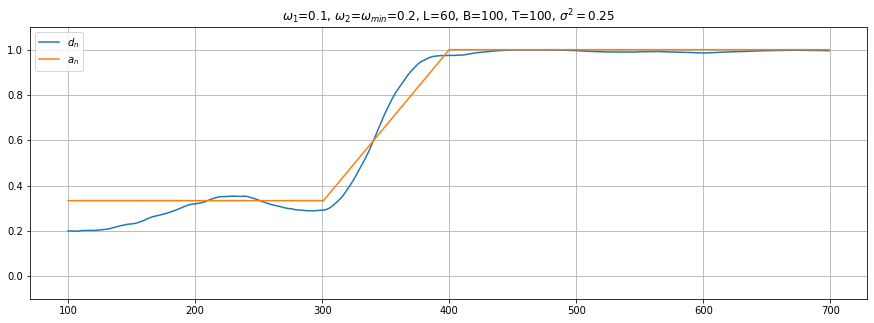
\includegraphics[width=1.0\linewidth]{row_linear_approximation_1.png}}
	\caption{Аппроксимация переходного интервала. Ряд с шумом, $ \Delta_{min} = 0.1 $.}
	\label{pic:row_linear_approximation_1}
\end{figure}

\begin{figure}[!hhh]
	\center{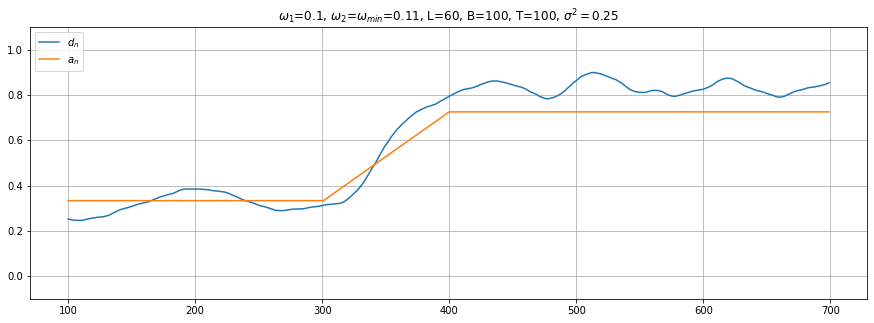
\includegraphics[width=1.0\linewidth]{row_linear_approximation_2.png}}
	\caption{Аппроксимация переходного интервала. Ряд с шумом, $ \Delta_{min} = 0.01 $.}
	\label{pic:row_linear_approximation_2}
\end{figure}

Важно отметить, что такая аппроксимация не всегда корректна (Рис. \ref{pic:row_linear_approximation_2}). В силу сходимости $ g_a $ к $ g $, у нас есть ограничения на $ L $. Однако аппроксимация прямой требует увеличения $ T - L $ и при уменьшении $ L $ возникает противоречие.

Поскольку мы хотим брать $ \gamma^* $ как значение в точке $ k $ прямой $ \gamma $, нам важно чтобы первые $ k $ значений $ \gamma $ были меньше $ d_n $, ведь в противном случае $ \hat{Q} > Q+k $. Таким образом на первый план выходит вопрос не только о корректности аппроксимации $ \gamma $ переходного интервала $ d_n $, но и о выборе доступных для изменения алгоритмом значений параметров $ B, T $ и $ L $. Позже попробуем установить их влияние на устойчивость системы.

\section{Алгоритм работы}
Таким образом, с учетом разделов \ref{ch:lower_border}, \ref{ch:apper_border} и \ref{ch:approx_d_n} уточним алгоритм \ref{algo:system_works}:

\begin{algorithm}\label{algo:system_works_final}
	Описание системы с учетом оценки $ \gamma $ и линейности переходного интервала функции $ d_n $:
	\begin{enumerate}
		\item Входные данные: $ F_N $, $ k $, $ \omega_1 $, $ \Delta_{min} $, $ \sigma^2 $;
		\item Результат: $ \hat{Q }$;
		\item Алгоритм:
		\begin{enumerate}
			\item Фиксируем $ B, T, L $;
			\item Оцениваем $ \gamma_{min} $ по формуле \eqref{eq:gamma_min};
			\item Вычисляем $ g_a(\omega_1, \omega_{min}) $ по формуле \eqref{eq:g_a};
			\item Строим прямую $ \gamma $, соединяющую $ \gamma_{min} $ и $ g_a(\omega_1, \omega_{min}) $;
			\item Фиксируем $ \gamma^* = \gamma(k) $;
			\item Определяем $ \hat{Q} $ как момент преодоления $ d_n $ значения $ \gamma^* $.
		\end{enumerate}	
	\end{enumerate}
\end{algorithm}

Дальнейшие исследования системы будут проводиться в соответствии с алгоритмом \ref{algo:system_works_final}.

\section{Оценка системы}
В дальнейших тестах дисперсия шума $ \sigma^2 = 0.25 $. 

Введем характеристики системы.

Будем считать, что произошло ложноположительное обнаружение неоднородности $ \mathrm{FP}(\gamma^*) $ при пороге $ \gamma^* $ если $ \hat{Q} < Q $. Если $ \hat{Q} \in [Q, Q+k] $ при пороге $ \gamma^* $, то у нас точное обнаружение $ \mathrm{TP}(\gamma^*) $. Если же $ \hat{Q} > Q+k $ для порога $ \gamma^* $, то произошло ложноотрицательное обнаружение неоднородности $ \mathrm{FN}(\gamma^*) $

Промоделируем $ n_{iter} $ раз реализацию шума $ \epsilon $ и на каждой итерации посчитаем $ \mathrm{FP}(\gamma^*) $, $ \mathrm{TP}(\gamma^*) $ и $ \mathrm{FN}(\gamma^*) $. Будем характеризовать систему вероятностью ложноположительного обнаружения $ \mathrm{FPR}(\gamma^*) = \frac{\sum\limits_{i=1}^{n_{iter}}\mathrm{FP}_i(\gamma^*)}{n_{iter}} $, вероятностью точного обнаружения $ \mathrm{TPR}(\gamma^*) = \frac{\sum\limits_{i=1}^{n_{iter}}\mathrm{TP}_i(\gamma^*)}{n_{iter}} $ и вероятностью ложноотрицательного обнаружения $ \mathrm{FNR}(\gamma^*) = \frac{\sum\limits_{i=1}^{n_{iter}}\mathrm{FN}_i(\gamma^*)}{n_{iter}} $.

Обозначим порог $ \gamma^* $, выбранный по алгоритму \ref{algo:system_works_final}, как $ \gamma_a $. Посчитаем $ \forall \gamma^* \in [0, 1] \;\newline \mathrm{FPR}(\gamma^*)$, $ \mathrm{TPR}(\gamma^*) $ и $ \mathrm{FNR}(\gamma^*) $. Также будем смотреть на $ \mathrm{FPR}(\gamma_a)$, $ \mathrm{TPR}(\gamma_a) $ и $ \mathrm{FNR}(\gamma_a) $.

\begin{figure}[!hhh]
	\center{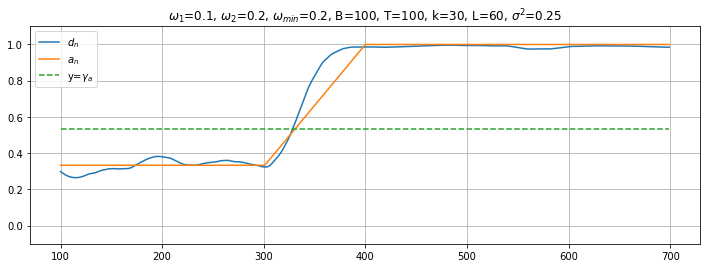
\includegraphics[width=1.0\linewidth]{system_estimation_one_iter.png}}
	\caption{Работы системы. Одна итерация, $ \sigma^2=0.25 $.}
	\label{pic:system_estimation_one_iter}
\end{figure}

\begin{figure}[!hhh]
	\center{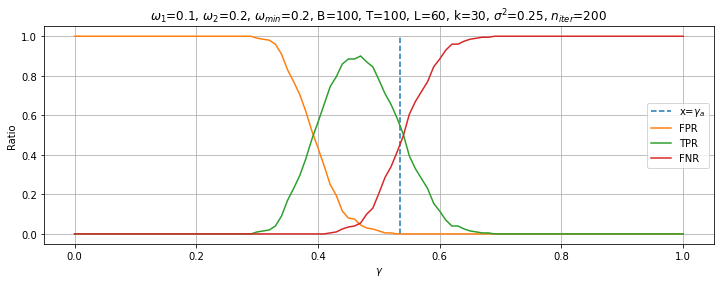
\includegraphics[width=1.0\linewidth]{system_estimation.png}}
	\caption{Работы системы. Оценка, $ \sigma^2=0.25 $.}
	\label{pic:system_estimation}
\end{figure}

Для параметров, указанных на Рис. \ref{pic:system_estimation}, $ \mathrm{FPR}(\gamma_a) = 0 $, $ \mathrm{TPR}(\gamma_a) = 0.585 $,  $ \mathrm{FNR}(\gamma_a) = 0.415 $. Исходя из этих значений, c вероятностью $ 0.415 $ предложенный алгоритм не справляется с требованием $ \hat{Q} \in [Q, Q+k] $.

При меньшей дисперсии шума $ \sigma^2 $ (Рис. \ref{pic:system_estimation_small_sd}, \ref{pic:system_estimation_small_sd_one_iter}), мы получаем большую устойчивость к ложноположительным обнаружениям, что позволяет уменьшить порог $ \gamma_a $ путем выбора значения на прямой $ \gamma $ раньше, чем в момент $ k $, так как при пороге $ \gamma_a $ остался процент запаздываний. Об этом нам говорит интервал значений $ \gamma(i) $ на Рис. \ref{pic:system_estimation_small_sd}, где вероятность точного обнаружения $ \mathrm{TPR}(\gamma(i)) = 1 $.


\begin{figure}[!hhh]
	\center{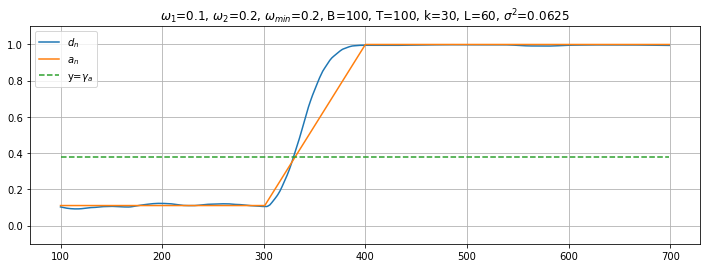
\includegraphics[width=1.0\linewidth]{system_estimation_small_sd_one_iter.png}}
	\caption{Работы системы. Одна итерация, $ \sigma^2=0.0625 $.}
	\label{pic:system_estimation_small_sd_one_iter}
\end{figure}

\begin{figure}[!hhh]
	\center{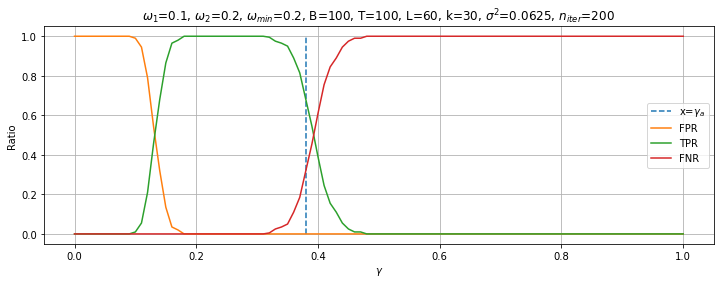
\includegraphics[width=1.0\linewidth]{system_estimation_small_sd.png}}
	\caption{Работы системы. Оценка, $ \sigma^2=0.0625 $.}
	\label{pic:system_estimation_small_sd}
\end{figure}



\section{Параметры системы}\label{sec:system_parameters}

Все параметры в системе, описываемой алгоритмом \ref{algo:system_works_final} можно разделить на $ 4 $ группы:
\begin{enumerate}
	\item Входные --- ряд и его характеристики до момента нарушения однородности: $ F_N, \omega_1, \sigma^2 $;
	\item Входные --- необходимые для работы алгоритма \ref{algo:system_works_final}: $ \Delta_{min}, k $;
	\item Неизвестные: $ \omega_2, Q $;
	\item Свободные, выбираемые системой: $ L, B, T $. Именно эти параметры мы можем подстраивать под разные ряды. Оценим их.
\end{enumerate}

\subsection{Оценка параметров: T}

При уменьшении параметра $ T $ длина переходного интервала сокращается, что увеличивает наклон прямой $ \gamma $ (Рис. \ref{pic:system_estimation_one_iter_t=70}), следовательно, порог $ \gamma_a $ имеет большее значения, что делает систему более устойчивой к шуму и при параметрах, указанных на Рис. \ref{pic:system_estimation_t=70} исключает ложноположительные обнаружения: $ \mathrm{FPR}(\gamma_a) = 0 $, $ \mathrm{TPR}(\gamma_a) = 0.99 $,  $ \mathrm{FNR}(\gamma_a) = 0.01 $.

\begin{figure}[!hhh]
	\center{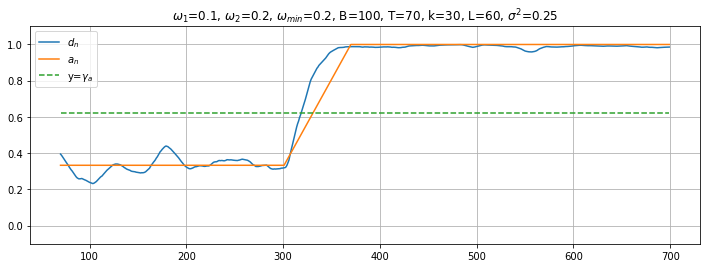
\includegraphics[width=\linewidth]{system_estimation_one_iter_t=70.png}}
	\caption{Работы системы. Одна итерация, $ T = 70 $.}
	\label{pic:system_estimation_one_iter_t=70}
\end{figure}

\begin{figure}[!hhh]
	\center{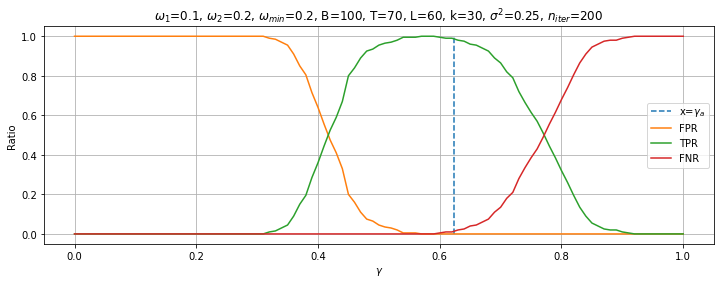
\includegraphics[width=\linewidth]{system_estimation_t=70.png}}
	\caption{Работы системы. Оценка, $ T = 70 $.}
	\label{pic:system_estimation_t=70}
\end{figure}

\newpage
При маленькой дисперсии шума $ \sigma^2 $ (Рис. \ref{pic:system_estimation_t=70_small_sd}), уменьшая $ T $ интервал значений $ \gamma(i) $, где вероятность точного обнаружения $ \mathrm{TPR}(\gamma(i)) = 1 $ становится еще больше, по сравнению с ситуацией на Рис. \ref{pic:system_estimation_small_sd}.

\begin{figure}[!hhh]
	\center{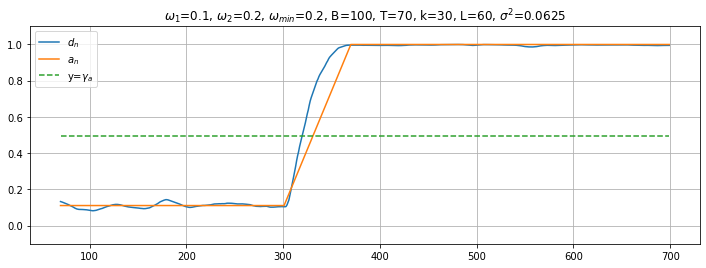
\includegraphics[width=\linewidth]{system_estimation_one_iter_t=70_small_sd.png}}
	\caption{Работы системы. Одна итерация, $ T = 70 $, $ \sigma^2=0.0625 $.}
	\label{pic:system_estimation_one_iter_t=70_small_sd}
\end{figure}

\begin{figure}[!hhh]
	\center{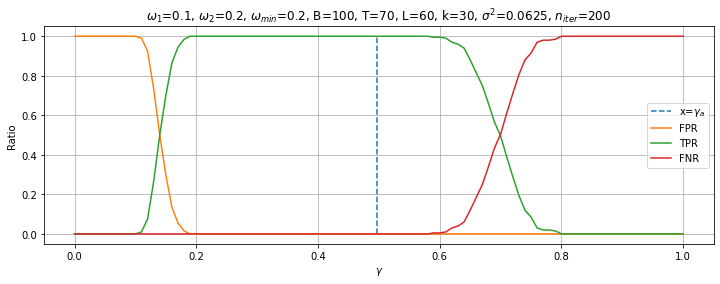
\includegraphics[width=\linewidth]{system_estimation_t=70_small_sd.png}}
	\caption{Работы системы. Оценка, $ T = 70 $, $ \sigma^2=0.0625 $.}
	\label{pic:system_estimation_t=70_small_sd}
\end{figure}


\newpage
При увеличении параметра $ T $ (Рис. \ref{pic:system_estimation_one_iter_t=130}) мы увеличиваем тестовый интервал, занижая параметр $ \gamma_a $, потенциально, делая систему менее устойчивой при большой дисперсии $ \sigma^2 $ шума $ \epsilon $. Также, при недостаточно высокой величине $ |T - L| $ линейная аппроксимация $ \gamma $ некорректна и первые значения $ \gamma $ превосходят значения $ d_n $ на переходном интервале, что влечет увеличение $ \mathrm{FNR}(\gamma_a) $.

При параметрах на Рис. \ref{pic:system_estimation_t=130}, $ \mathrm{FPR}(\gamma_a) = 0 $, $ \mathrm{TPR}(\gamma_a) = 0.265 $, $ \mathrm{FNR}(\gamma_a) = 0.735 $. Получили, что с вероятностью в $ 0.735 $ требование $ \hat{Q} \in [Q, Q+k] $ будет нарушено.


\begin{figure}[!hhh]
	\center{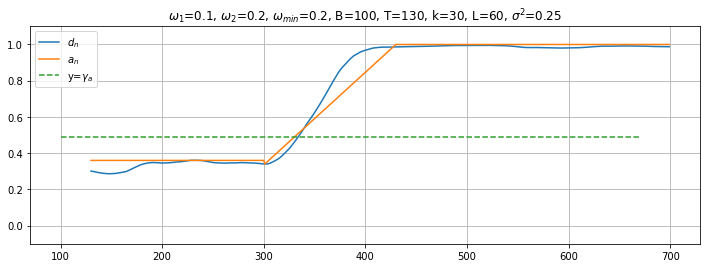
\includegraphics[width=\linewidth]{system_estimation_one_iter_t=130.png}}
	\caption{Работы системы. Одна итерация, $ T = 130 $.}
	\label{pic:system_estimation_one_iter_t=130}
\end{figure}

\begin{figure}[!hhh]
	\center{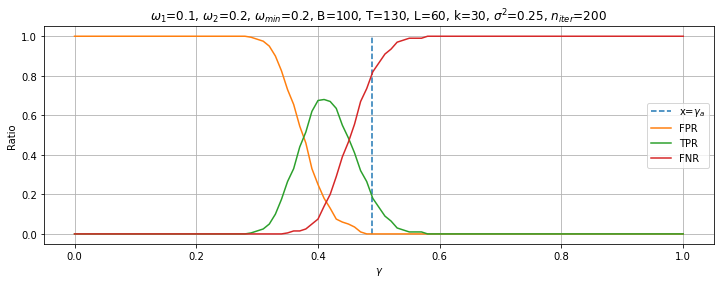
\includegraphics[width=\linewidth]{system_estimation_t=130.png}}
	\caption{Работы системы. Оценка, $ T = 130 $.}
	\label{pic:system_estimation_t=130}
\end{figure}

\newpage
Таким образом, уменьшая $ T $, мы увеличиваем устойчивость системы, а также интервал $ k_{rob}, \; k_{rob} < k $, на котором $ \forall i: \mathrm{TPR}(\gamma(i)) = 1 $, следствием чего является $ \hat{Q} \rightarrow Q $ --- более точное обнаружение момента нарушения однородности.

Однако, при $ T \rightarrow L $, $ K_{test} \rightarrow 1 $, и вклад шума в значения $ d_n $ увеличивается, что влечет увеличение ложноположительных обнаружений (Рис. \ref{pic:decreasing_T}). 

Также было эмпирически установлено, что при уменьшении $ T - L $ скорость роста переходного интервала становится быстрее линейной.

\begin{figure}[!hhh]
	\center{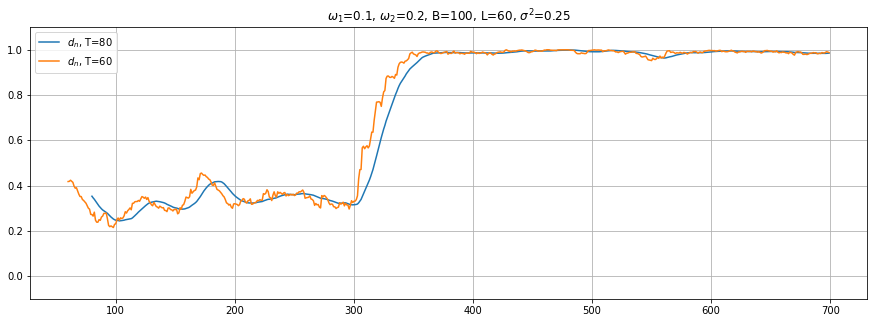
\includegraphics[width=1.0\linewidth]{decreasing_T.png}}
	\caption{Функция $ d_n $. Уменьшение $ T - L $.}
	\label{pic:decreasing_T}
\end{figure}

Как было отмечено ранее, близость $ g_a $ к $ g $ имеет место при достаточно большом $ L $, однако линейность переходного интервала достигается при противоположном условии. Получается противоречие, так как при увеличении $ L $, количество векторов вложений $ n_Q $, содержащих момент возмущения, также возрастет, и при фиксированном $ T $ равенство в формуле \eqref{eq:linear_g} достигаться не будет в силу $ n_Q = O(L) $. Линейность переходного интервала нарушается, однако скорость роста при уменьшении $ T - L $ становится быстрее линейной (Рис. \ref{pic:decreasing_T} и \ref{pic:row_diff_L}). 

\begin{figure}[!hhh]
	\center{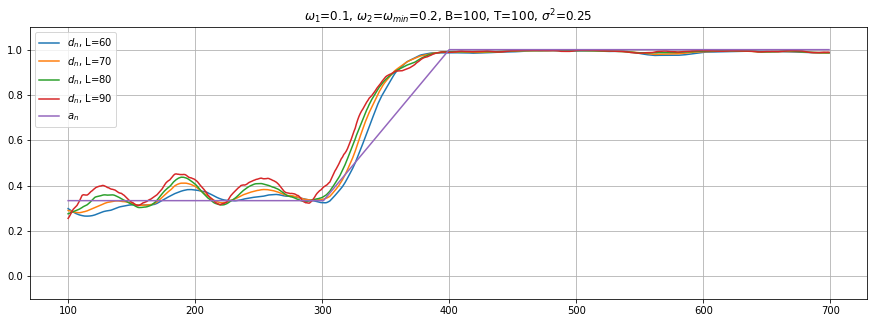
\includegraphics[width=1.0\linewidth]{row_diff_L.png}}
	\caption{Функция $ d_n $. Разные значения $ L $.}
	\label{pic:row_diff_L}
\end{figure}

\newpage
\subsection{Оценка параметров: B}
Параметр $ B $ влияет на устойчивость системы и его уменьшение может увеличить значение $ \mathrm{FPR}(\gamma^*) $. Чем больше $ B $, тем точнее определяется базовое пространство $ \mathfrak{L_r^{(1)}} $ (Рис. \ref{pic:row_diff_small_B}, \ref{pic:row_diff_big_B}) и до момента $ Q $ значения $ d_n $ имеют меньший разброс.
\begin{figure}[!hhh]
	\center{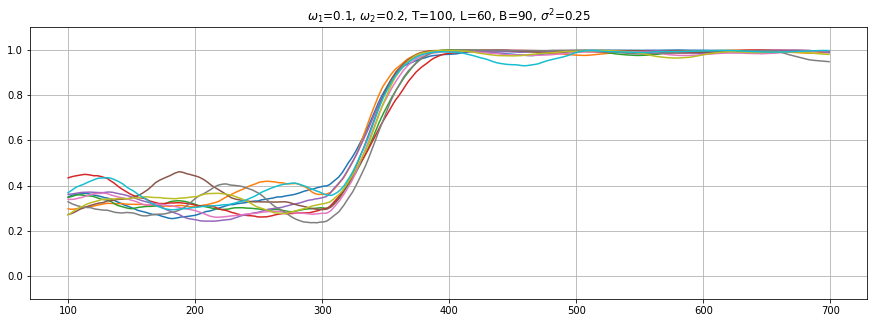
\includegraphics[width=1.0\linewidth]{row_diff_small_B.png}}
	\caption{Функция $ d_n $. Реализации шума, $ B=90 $.}
	\label{pic:row_diff_small_B}
\end{figure}

\begin{figure}[!hhh]
	\center{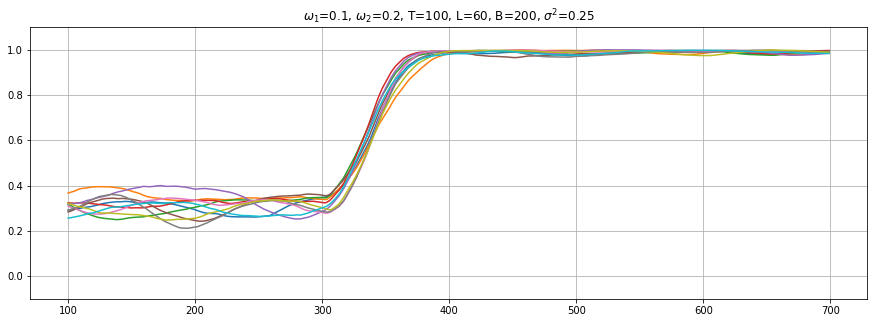
\includegraphics[width=1.0\linewidth]{row_diff_big_B.png}}
	\caption{Функция $ d_n $. Реализации шума, $ B=200 $.}
	\label{pic:row_diff_big_B}
\end{figure}

\section{Обобщение}\label{sec:generalization}
Описанную алгоритмом \ref{algo:system_works_final} систему использовать на практике проблематично из-за требований к вводу пользователем дисперсии шума $ \sigma^2 $ и частоты периодики $ \omega_1 $. Внесем оценку этих входных параметров в работу алгоритма.

\subsection{Упрощение: $ \sigma^2 $}
Добавим требование к входному ряду $ F_N $ --- первые $ \frac{N}{4} $ элементов ряда гарантированно не содержат разладку. Можно это расценивать как наличие неких исторических данных, в которых структура ряда не менялась. Таким образом, в качестве $ \gamma_{min} $ будем брать максимальное значение строковой функции неоднородности, оцененное на первых $ \frac{N}{4} $ элементах ряда $ F_N $. Обозначим этот подряд как $ F_N^{(h)} $.

\subsection{Упрощение: $ \omega_1 $}
Начальную частоту периодики мы можем оценить используя пакет $ \mathrm{RSSA} $:
\begin{algorithm}\label{algo:estimate_omega_1}
	Оценка начальной частоты ряда $ \omega_1 $:
	\begin{enumerate}
		\item Строим траекторную матрицу ряда $ F_N^{(h)} $;
		\item Применяем к ней $ \mathrm{SVD} $ - разложение;
		\item Группируем компоненты на основе матрицы взвешенных корреляций;
		\item Используем алгоритм $ \mathrm{ESPRIT} $ для оценки компонент $ \mathrm{LRR} $ для сигнала;
		\item Выбираем компоненты, отвечающие за периодику и оцениваем частоту.	
	\end{enumerate}
\end{algorithm}

При тестировании реализации алгоритма \ref{algo:estimate_omega_1} $ \forall n \in [3, \frac{N}{4}]: \omega_1 = \frac{1}{n}$ для рядов без шума и для белого шума со стандартным отклонением $ \sigma \in [0.1, 0.8] $ ошибок в оценке $ \omega_1 $ не было. 

При добавление линейного тренда вида $ kx + b $, ошибка оценки не превышала значение $ 0.02 $ для $ k \in [0.01, 0.5] $.

\section{Упрощенный алгоритм}
Исходя из раздела \ref{sec:generalization}, опишем новый алгоритм.
\begin{algorithm}\label{algo:system_simplification}
	Описание системы:
	\begin{enumerate}
		\item Входные данные: $ F_N $, $ k $, $ \Delta_{min} $;
		\item Результат: $ \hat{Q}$;
		\item Алгоритм:
		\begin{enumerate}
			\item Фиксируем $ B, T, L $;
			\item Оцениваем $ \omega_1 $ по алгоритму \ref{algo:estimate_omega_1};
			\item Оцениваем $ \gamma_{min} $ как максимум функции $ d_n $ на промежутке $ [0; \frac{N}{4} - T] $;
			\item Вычисляем $ g_a(\omega_1, \omega_{min}) $ по формуле \eqref{eq:g_a};
			\item Строим прямую $ \gamma $, соединяющую $ \gamma_{min} $ и $ g_a(\omega_1, \omega_{min}) $;
			\item Фиксируем $ \gamma^* = \gamma(k) $;
			\item Определяем $ \hat{Q} $ как момент преодоления $ d_n $ значения $ \gamma^* $.
		\end{enumerate}
	\end{enumerate}
\end{algorithm}


\section{Тестирование}
Исходя из результатов секции \ref{sec:system_parameters}, мы получили общую идею для выбора параметров $ B, T, L $ --- система имеет большую устойчивость в смысле вероятности точного определения момента нарушения однородности $ \mathrm{TPR}(\gamma^*) $ при большом $ B, L $ и маленьком значении $ T - L $. 

Поскольку представление о длине ряда в алгоритме \ref{algo:system_simplification} мы получаем только из входного параметра $ F_N $, а также с учетом требования ко входному ряду о гарантированном отсутствии неоднородности в первых $ \frac{N}{4} $ элементах, положим $ B = \lfloor \frac{N}{6} \rfloor,\; T = B,\; L = 0.9 \cdot T $.

Ниже приведены результаты тестирования системы.


\newpage
\chapter*{Заключение}
\addcontentsline{toc}{chapter}{Заключение}

В данной работе были рассмотрены и сравнены функции обнаружения неоднородности в синусоидальных временных рядах с неоднородностями, заданными изменением частоты, амплитуды, фазовым сдвигом и выбросом. 

Был тщательно рассмотрен и аналитически упрощен индекс неоднородности \newline $ g(F^{(1)}, F^{(2)}) $. Для аналитической аппроксимации $ g_a $ были приведены численные эксперименты, подтверждающие хорошее качество полученной аппроксимации при достаточно большой длине окна $L$.

Была разработана система автоматического обнаружения неоднородности за указанный временной интервал после неизвестной точки разладки на основе анализа поведения функции неоднородности на переходном интервале.

Анализ показал, что алгоритм построения порога нуждается в доработке с учетом нелинейности функции разладки. Однако, в случае правильного выбора параметров, в частности, $ Т $ и $ L $, алгоритм работает хорошо с точки зрения малого количества ложных срабатываний и запаздываний при обнаружении разладки.


\bibliographystyle{gost2008}
\bibliography{report.bib}
\end{document}